\documentclass[graybox]{svmult}

% choose options for [] as required from the list
% in the Reference Guide

\usepackage{mathptmx}       % selects Times Roman as basic font
\usepackage{helvet}         % selects Helvetica as sans-serif font
\usepackage{courier}        % selects Courier as typewriter font
\usepackage{type1cm}        % activate if the above 3 fonts are
                             % not available on your system
%
\usepackage{makeidx}         % allows index generation
\usepackage{graphicx}        % standard LaTeX graphics tool
                             % when including figure files
\usepackage{multicol}        % used for the two-column index
\usepackage[bottom]{footmisc}% places footnotes at page bottom
\usepackage{latexsym,amsmath,amssymb,bm,booktabs,epsfig,multirow,bigstrut,graphicx,url,xspace,natbib}
%\usepackage{nath}

% see the list of further useful packages
% in the Reference Guide

\makeindex             % used for the subject index
                       % please use the style svind.ist with
                       % your makeindex program
                       
\input FJHDef.tex
%\renewcommand{\bvec}[1]{\textbf{\itshape #1}}
%\renewcommand{\bvec}[1]{\boldsymbol{#1}}
\newcommand{\cube}{[0,1)^d}
\newcommand{\tcube}{\widetilde{[0,1)}^d}
\newcommand{\hv}{\hat{v}}
\newcommand{\fudge}{\mathfrak{C}}
\DeclareMathOperator{\MSE}{MSE}
\DeclareMathOperator{\RMSE}{RMSE}
\DeclareMathOperator{\rnd}{rnd}
\DeclareMathOperator{\abso}{abs}
\DeclareMathOperator{\rel}{rel}
\DeclareMathOperator{\nor}{nor}
\DeclareMathOperator{\err}{err}
%\DeclareMathOperator{\prob}{prob}
\DeclareMathOperator{\third}{third}
\DeclareMathOperator{\qse}{qse}
\DeclareMathOperator{\card}{card}
%\DeclareMathOperator{\fourth}{fourth}
%\newtheorem{theorem}{Theorem}
\newtheorem{prop}[theorem]{Proposition}
%\newtheorem{rem}{Remark}
\DeclareMathOperator{\sMC}{sMC}
\newcommand{\aMC}{{\tt cubMC}\xspace}
\begin{document}


\date{\today}
\title*{Automatic Monte Carlo Algorithms Where the Integrand Size Is Unknown
\thanks{The first and second authors were partially supported by the National
Science Foundation under DMS-0923111 and DMS-1115392}}
\titlerunning{Adaptive Monte Carlo}
\author{Fred J. Hickernell\inst{1} \and
Lan Jiang\inst{1} \and Yuewei Liu\inst{2} \and Art Owen \inst{3}}
\institute{Department of Applied Mathematics,
Illinois Institute of Technology, Chicago, IL, USA,
\texttt{hickernell@iit.edu,ljiang14@hawk.iit.edu}
\and
School of Mathematics and Statistics, Lanzhou University, Lanzhou City, Gansu, China 730000, \texttt{???}
\and 
Art's address here \texttt{with email here}
}
%
% Use the package "url.sty" to avoid
% problems with special characters
% used in your e-mail or web address
%
\maketitle

\abstract{{\bf When we are done, we will write this.}}


\section{Introduction}

Monte Carlo algorithms for multidimensional integrals have been in use for half a century.  The integral or mean, $\mu$, of a $d$-variate function $f: \reals^d \to \reals$, i.e.,
\begin{equation*} 
\mu= \mu(f) = \int_{\reals^d} f(\vx) \rho(\vx) \, \dif \vx,
\end{equation*}
is approximated by the sample mean of integrand values,
\begin{equation} \label{samplemean}
\hmu_n = \frac 1n \sum_{i=1}^n Y_i, \qquad Y_i = f(\vX_i).
\end{equation}
Here $\rho: \reals^d \to [0,\infty)$ is a specified probability density function, e.g., the uniform density on a cube or the normal density.  For simple Monte Carlo the points $\vX_1, \vX_2, \ldots$ independent and identically distributed (i.i.d.) random variables with the marginal probability density function $\rho$.  Other choices, such as quasi-random points, may provide greater accuracy, but this paper deals with only simple Monte Carlo.

It is natural to that practitioners would want an automatic Monte Carlo algorithm that takes as its input the integrand, $f$, the probability density, $\rho$, and an error tolerance $\varepsilon$, and produces a value $\hmu_n$ that is within $\varepsilon$ of $\mu$ while requiring only a reasonable sample size, $n$.  While there is an extensive theory on Monte Carlo algorithms, there are some key gaps that must be filled to make it an automatic algorithm.  The aim of this article is to provide such an algorithm.  Next this problem of approximating $\mu$ is summarized from the perspective of a statistician and then from the perspective of an information-based complexity theorist or numerical analyst.

{\bf Art will add and edit this material in this section, especially the next subsection.}

\subsection{The Statistician's Perspective} \label{statperspsec}  
The statistician's sees this a problem of constructing non-parametric, fixed-width confidence intervals for $\mu$.  Setting $Y=f(\vX)$, the goal is to approximate its mean, $\mu=E(Y)$, from an i.i.d.\ sample, $Y_i=f(\vX_i)$, $i=1, \ldots, n$, to obtain an expression
\begin{equation} \label{abserr}
\Prob\left[\abs{\hmu_n-\mu} \le \varepsilon \right] \geq 1-\alpha.
\end{equation}
Here taking $\alpha=5\%$ corresponds to a $95\%$ confidence interval for $\mu$ with half-width $\varepsilon$.  Although the probability distribution for $Y$ is not readily obtainable, the Central Limit Theorem states that the sample mean, $\hmu_n$, is approximately normally distributed for large $n$.  This fact may be used to determine the sample size $n$ to give an approximate confidence interval, 
\begin{equation} \label{CLT}
\Prob\left[\abs{\hmu_n-\mu} \le \frac{z_{\alpha/2} \sigma} {\sqrt{n}} \right] \approx 1-\alpha,
\end{equation}
where $\sigma^2 = \var(Y)=E[(Y-\mu)^2]$, and $z_\alpha$ denotes the $(1-\alpha)100\%$ percentile of the standard Gaussian distribution.  This suggests taking a sample size of $n=\lceil (z_{\alpha/2}\sigma/\varepsilon)^2\rceil$ to attain \eqref{abserr}.  Since $\sigma$ is not known a priori, it must be approximated by the sample variance of the $Y_i$:
\begin{equation} \label{samplevar}
\hsigma^2 = \fudge^2 \hv_{n_{\sigma}}, \quad \text{where} \quad \hv_{n_{\sigma}} = \frac 1{n_{\sigma}-1} \sum_{i=1}^{n_{\sigma}} (Y_i- \hmu_{n_{\sigma}})^2, \quad \hmu_{n_{\sigma}} = \frac 1{n_{\sigma}} \sum_{i=1}^{n_{\sigma}} Y_i.
\end{equation}
The variance inflation factor, $\fudge>1$, accounts for the fact the unbiased variance estimator, $\hv_{n_{\sigma}}$, may be larger or smaller than the true variance, $\sigma^2$.  Then the sample size for the sample mean may be chosen as $n=\lceil (z_{\alpha/2}\hsigma/\varepsilon)^2\rceil$.  To avoid dependence between $\hsigma^2$ and $\hmu_n$, an independent sample of $Y_i$, should be used to compute $\hmu_n$, i.e., 
\begin{equation} \label{simpleMCest}
\hmu_n = \frac 1n \sum_{i=n_{\sigma}+1}^{n_{\sigma}+n} Y_i,
\end{equation}
for a total cost of $n_{\sigma}+n$ samples.

While this fixed-width confidence interval may be often correct, it is not guaranteed. There are two approximations, whose errors must be understood and controlled: approximating the distribution $\hmu_n$ as a Gaussian distribution, and approximating $\sigma^2$ by the sample variance.  The key to controlling these two errors, as seen in Theorem \ref{mainadaptthm}, is in assuming a bound on the kurtosis, i.e., 
\begin{equation} \label{boundedkurt}
\kappa=\kurt(Y) = \frac{E[(Y-\mu)^4]}{\sigma^4} \le \kappa_{\max}.
\end{equation}
(Note, sometimes in the literature, the kurtosis is defined as the expression above minus three.)  A bounded kurtosis means that $Y$ has or does not have ????? {\bf help Art}. A bounded kurtosis allows one to reliably bound $\var(Y)$ in terms of the sample variance, and also allows one to obtain a rigorous bound on the deviation of the sample mean from the true mean.  It was shown by \cite[Corollary 2]{BahSav56} that nonparametric confidence intervals are impossible for convex sets of distributions. Assuming bounded kurtosis produces a non-convex set of possible distributions for $Y$.

Another approach to obtaining a fixed-width confidence interval for $\mu$ would be to assume an upper bound on $\sigma^2$ and apply Chebyshev's inequality.  The disadvantage of this approach is that while it might work for $Y=f(\vX)$, it would not work for $cY=cf(\vX)$ if $c$ were large enough, since $\var(cY)=c^2 \var(Y)$.  However, since $\kurt(cY)=\kurt(Y)$ if the procedure for obtaining a fixed-width confidence interval that is described in this article works for $Y$, it also works for $cY$.

\subsection{The Information-Based Complexity Theorist's or Numerical Analyst's Perspective} 
The information-based complexity theorist or numerical analyst sees this as a multivariate integration problem.  There are a myriad of cubature methods, each making certain assumptions on the domain of integration and the smoothness of the integrand, $f$, and deriving error bounds in terms of some semi-norm of $f$. Simple Monte Carlo methods work for functions with low degrees of smoothness and the natural space of integrands is $\cl_2$, where the $\cl_{p}$ norm is defined as
\begin{equation} \label{Lpnormdef}
\norm[p]{f} :=\left\{\int_{\reals^d} \abs{f(\vx)}^p \rho(\vx) \, \dif \vx\right\}^{1/p}.
\end{equation}
The root mean square error of the simple Monte Carlo method is $\norm[2]{f-\mu(f)}/\sqrt{n}$.

Again, the practical problem again in applying this error analysis to determine the sample size, $n$, to guarantee the desired error, one must know the size of the integrand, $\norm[2]{f-\mu(f)}=\sqrt{\var(Y)}=\sigma$.  Analogous to the statistical argument given above, the solution to this problem is not to look at balls of integrands, i.e., 
\begin{equation} \label{ballintegdef}
\cb_{\sigma_{\max}} = \{ f \in \cl_2 : \norm[2]{f-\mu(f)} \le \sigma_{\max}\}, 
\end{equation}
but to look at \emph{cones} of integrands 
\begin{equation}\label{coneintegdef}
\cc_{\kappa_{\max}} = \{f \in \cl_4 : \norm[4]{f-\mu(f)} \le \kappa_{\max}^{1/4} \norm[2]{f-\mu(f)} \}.
\end{equation}
This condition is the same as \eqref{boundedkurt}.  Whereas $f$ lying in the ball  $\cb_{\sigma_{\max}}$ does not guarantee $cf$ lies in that same ball, $f$ lying in the cone $\cc_{\kappa_{\max}}$, does guarantee that $cf$ lies in that same cone.

Looking for algorithms that work well for cones of integrands, $\cc_{\kappa_{\max}}$, leads one to \emph{adaptive} algorithms.  The sample size used to estimate the integral is determined adaptively by first computing an upper bound on $\norm[2]{f-\mu(f)}$.  In information-based complexity theory it is known that adaptive information does not help for convex sets of integrands in the worst case and probabilistic settings \citep[Chapter 4, Theorem 5.2.1; Chapter 8, Corollary 5.3.1]{TraWasWoz88}.  Here, the cone, $\cc_{\kappa_{\max}}$ is not a convex set, so adaption can help.

Again, it should be stressed that the algorithm to be presented here is automatic.  It does not require information about $\norm[2]{f-\mu(f)}=\sigma$, but this quantity needs to be reliably estimated by the algorithm. Thus, the sample size needed, and consequently the time required, to estimate $\mu$ to within the prescribed error tolerance depends on how large $\norm[2]{f-\mu(f)}=\sigma$ is estimated to be.  The algorithm is adaptive, and its cost depends on the integrand.

\subsection{Illustrative Univariate Examples of Automatic Algorithms}

Several commonly used software packages have automatic algorithms for integrating functions of a single variable.  These include 
\begin{itemize} 

\item {\tt quad} in MATLAB \citep{MAT7.12}, adaptive Simpson's rule based on {\tt adaptsim} by \cite{GanGau00a},

\item {\tt quadgk} in MATLAB \citep{MAT7.12}, adaptive Gauss-Kronrod quadrature based on {\tt quadva} by \cite{Sha08a}, and

\item the {\tt chebfun} \citep{TrefEtal12} toolbox for MATLAB \citep{MAT7.12}, which approximates integrals by integrating interpolatory Chebyshev polynomial series for the integrands.

%\item {\tt NIntegrate} in Mathematica \citep{Mat8a}, which uses a number of adaptive rules for one dimensional integrals, 

\end{itemize}

For the first three of these automatic algorithms one can easily probe where they sample the integrand, feed the algorithms zero values, and then construct fooling functions that the automatic algorithms will return a zero value for the integral.  Figure \ref{foolfunfig} displays these fooling functions for the problem $\mu=\int_0^1 f(x) \, \dif x$ for the first three algorithms. Each of these algorithms is asked to provide an answer with an absolute error no greater than $10^{14}$, but in fact the the absolute error is $1$ for these fooling functions.  The algorithms {\tt quad} and {\tt chebfun} sample only about a dozen points before concluding that the function is zero, whereas the algorithm {\tt quadgk} samples a much larger number of points (only those between $0$ and $0.01$ are shown in the plot). Algorithm {\tt NIntegrate} is hard snoop, but it is examined for the next example.

\begin{figure}
\centering
\begin{minipage}{3.7cm} \centering 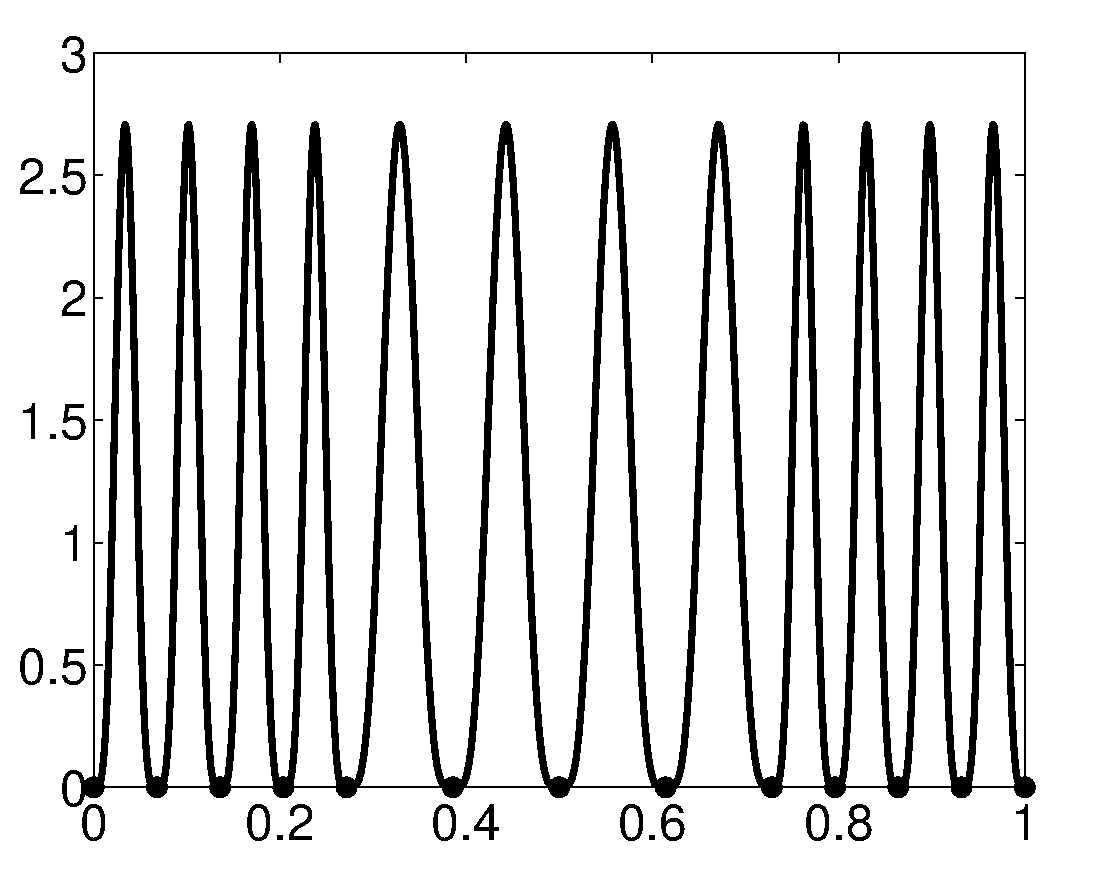
\includegraphics[width=3.7cm]{Foolquadbw.eps} \\ {\tt quad} \end{minipage}
\begin{minipage}{3.7cm} \centering 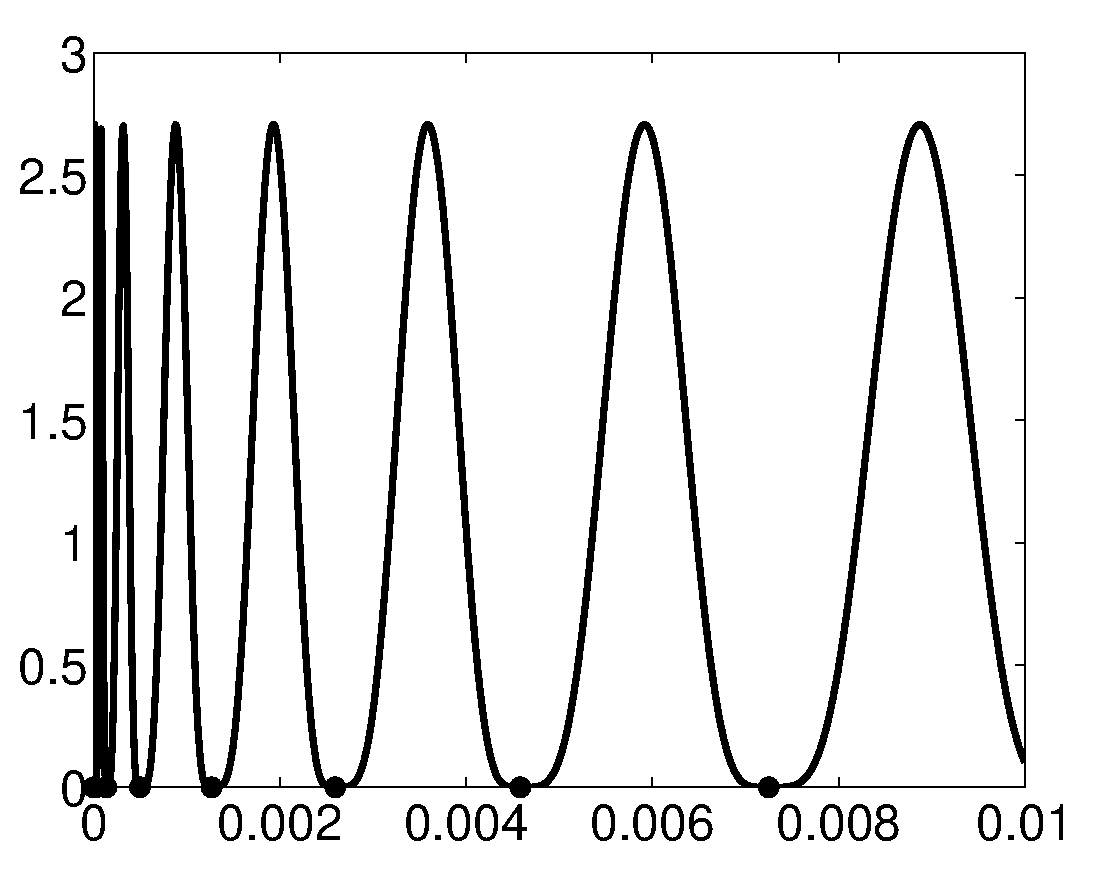
\includegraphics[width=3.7cm]{Foolquadgkbw.eps} \\ {\tt quadgk} \end{minipage}
\begin{minipage}{3.7cm} \centering 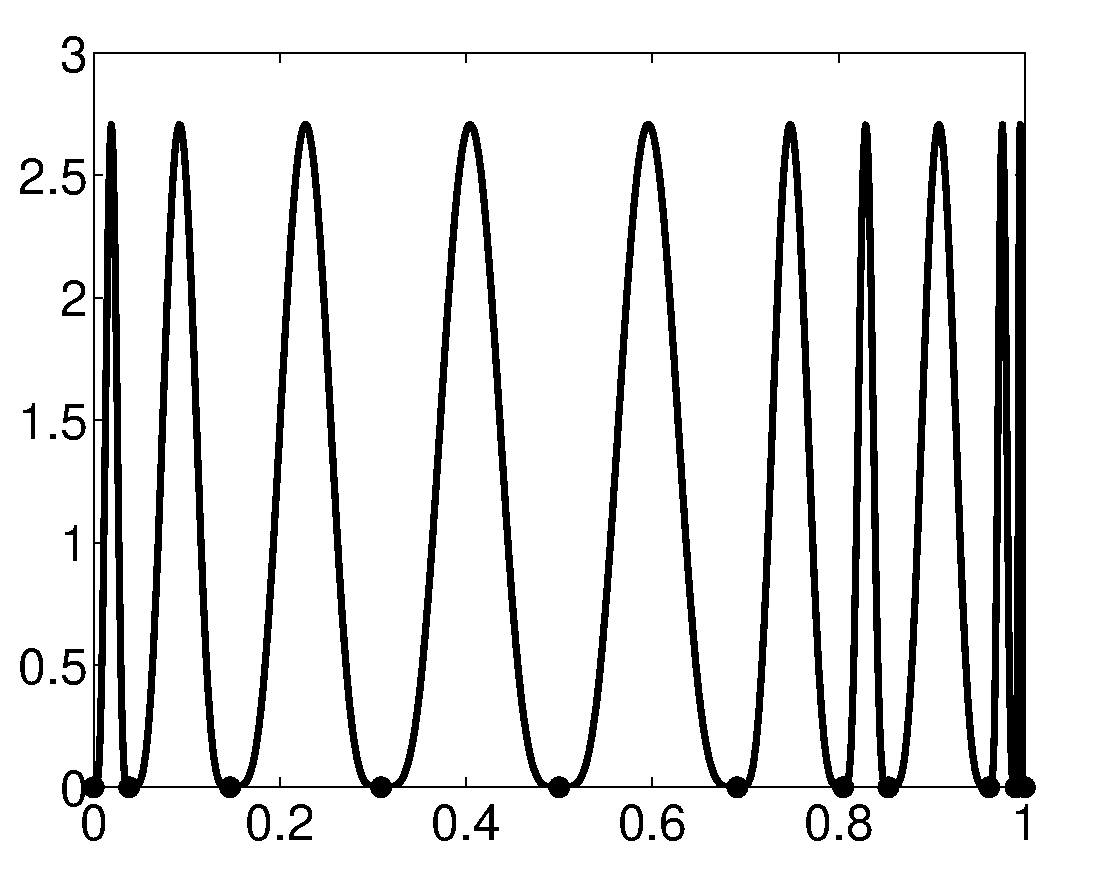
\includegraphics[width=3.7cm]{Foolchebintbw.eps} \\ {\tt chebfun} \end{minipage}
\caption{Plots of fooling functions, $f$, with $\mu=\int_0^1 f(x) \, \dif x=1$, but for which the corresponding algorithms return values of $\hmu=0$. \label{foolfunfig}}
\end{figure}


Accuracy and timing results have been recorded for the test function
\begin{equation} \label{GaussianTestFun}
f(\vx)=a_0 + b_0\prod_{j=1}^d\left[ 1 +b_j \exp \left(-\frac{(x_j-h_j)^2}{c_j^2}\right) \right].
\end{equation}
Here $\vx$ is a $d$ dimensional vector, and the $b_j$, $c_j$, and $h_j$ are parameters.  For Figure \ref{GaussianTestFunFig} shows the results of different algorithms being used to integrate $500$ different instances of $f$.  For each instance of $f$, the parameters are chosen as follows:
\begin{itemize} 
\item $b_j \in [0.1,1]$ with $\log(b_j)$ being i.i.d.\ uniform, $j=1, \ldots, d$,
\item $c_j \in [10^{-6},1]$ with $\log(c_j)$ being i.i.d.\ uniform, $j=1, \ldots, d$,
\item $h_j \in [0,1]$ with $h_j$ being i.i.d.\ uniform, $j=1, \ldots, d$,
\item $b_0$ chosen in terms of the $b_j$, $c_j$, and $h_j$ in order to make $\sigma^2(f) \in [10^{-2}, 10^2]$, with $\log(\sigma(f))$ being i.i.d.\ uniform for each instance, and
\item $a_0$ in terms of chosen in terms of the $b_j$, $c_j$, and $h_j$ to make $\mu(f)=1$.
\end{itemize}

\begin{figure}
\centering
\begin{minipage}{5.7cm} \centering 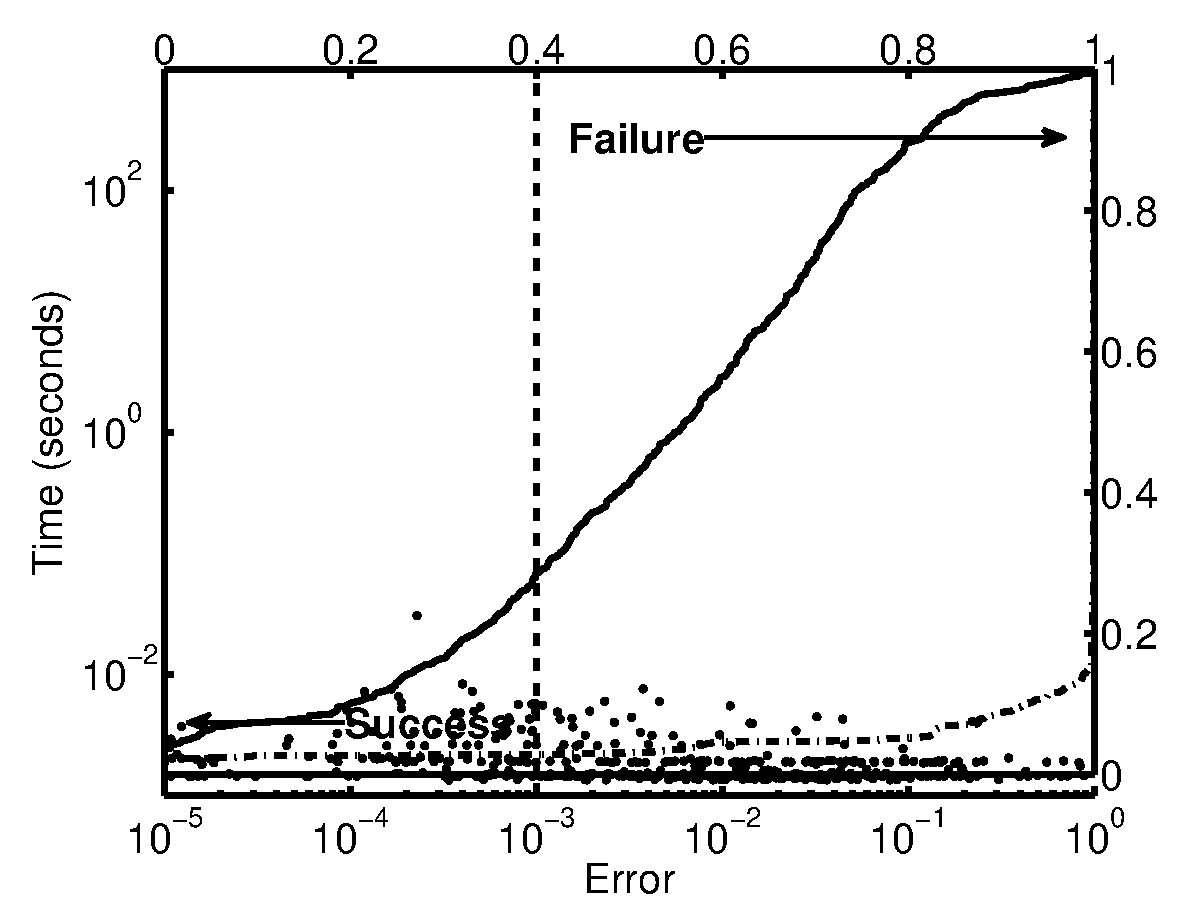
\includegraphics[width=5.7cm]{gaussiand=1quadErrTime.eps} \\ {\tt quad} \end{minipage}
\begin{minipage}{5.7cm} \centering 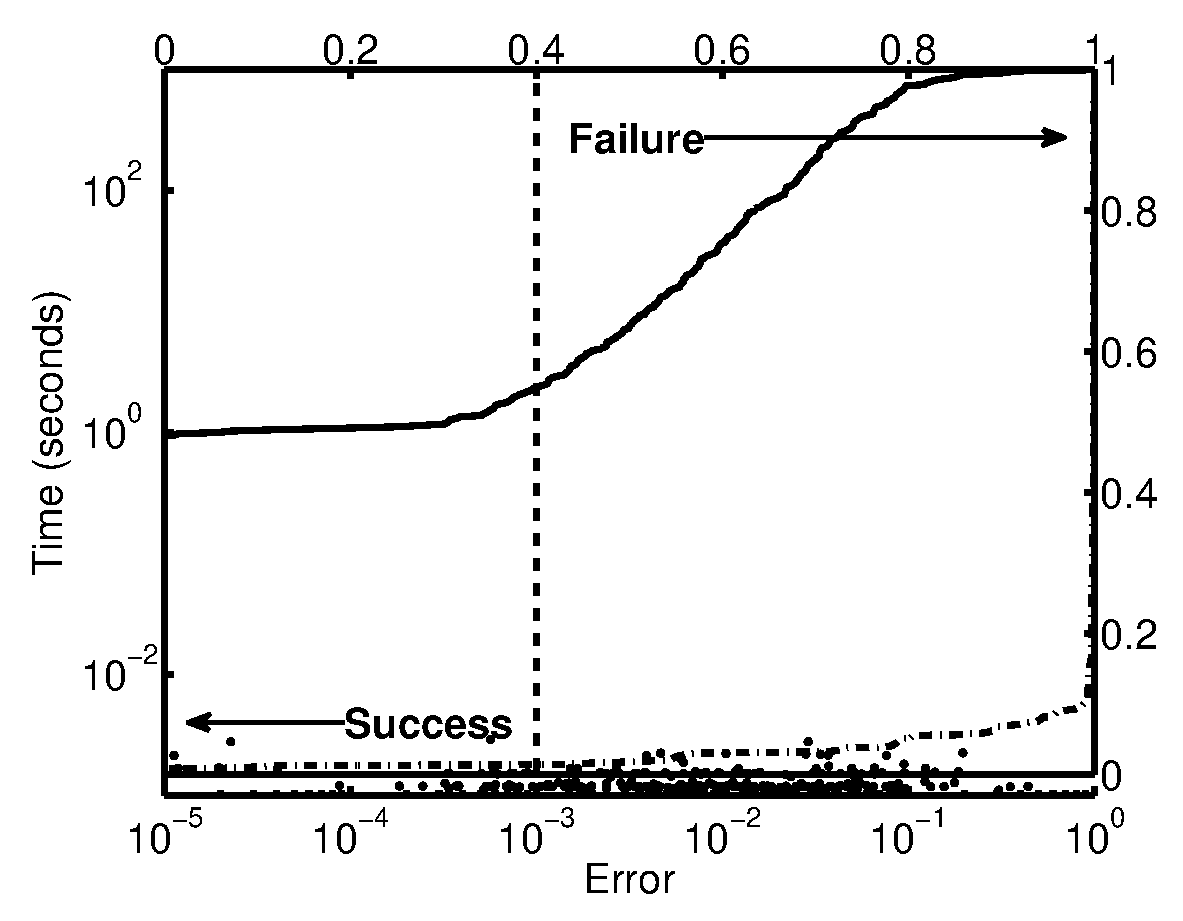
\includegraphics[width=5.7cm]{gaussiand=1quadgkErrTime.eps} \\ {\tt quadgk} \end{minipage}
\begin{minipage}{5.7cm} \centering 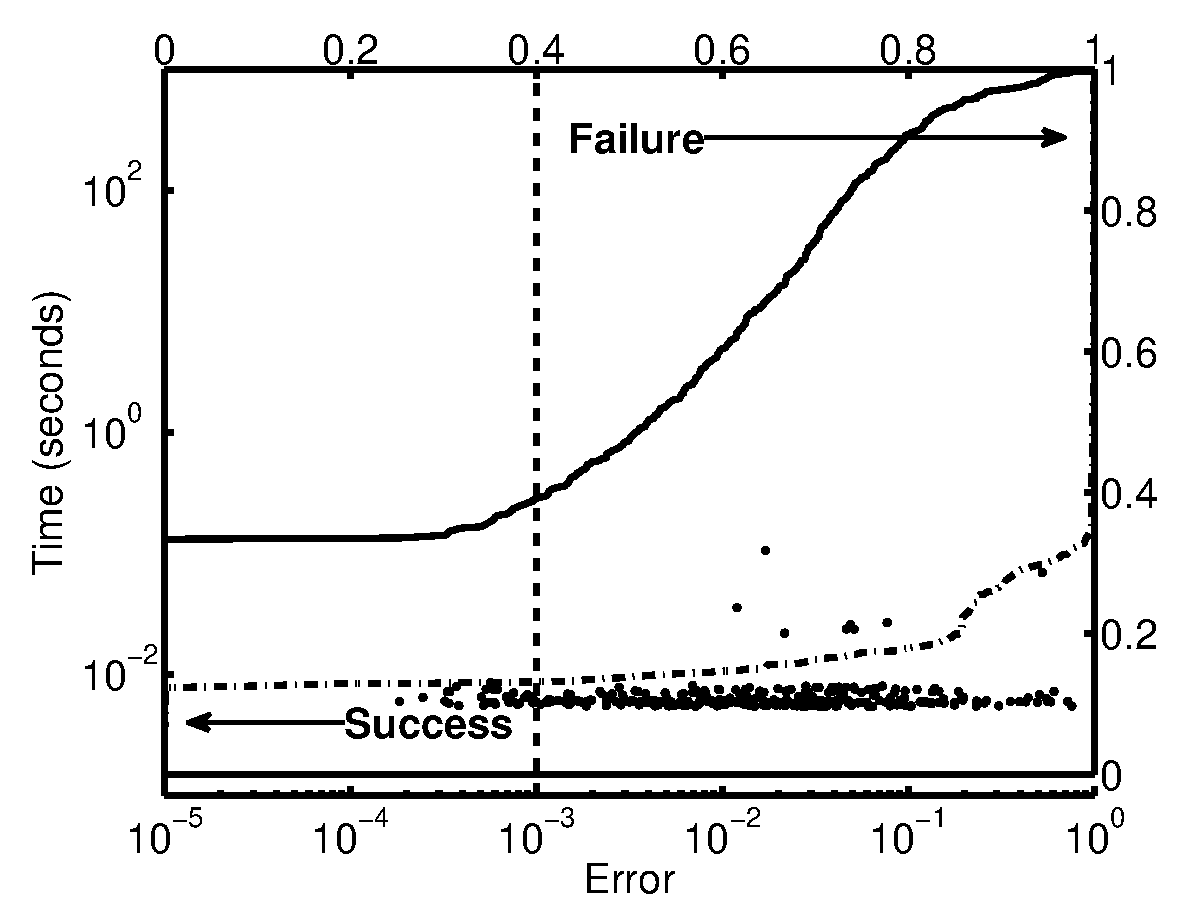
\includegraphics[width=5.7cm]{gaussiand=1chebfunErrTime.eps} \\ {\tt chebfun} \end{minipage}
\begin{minipage}{5.7cm} \centering 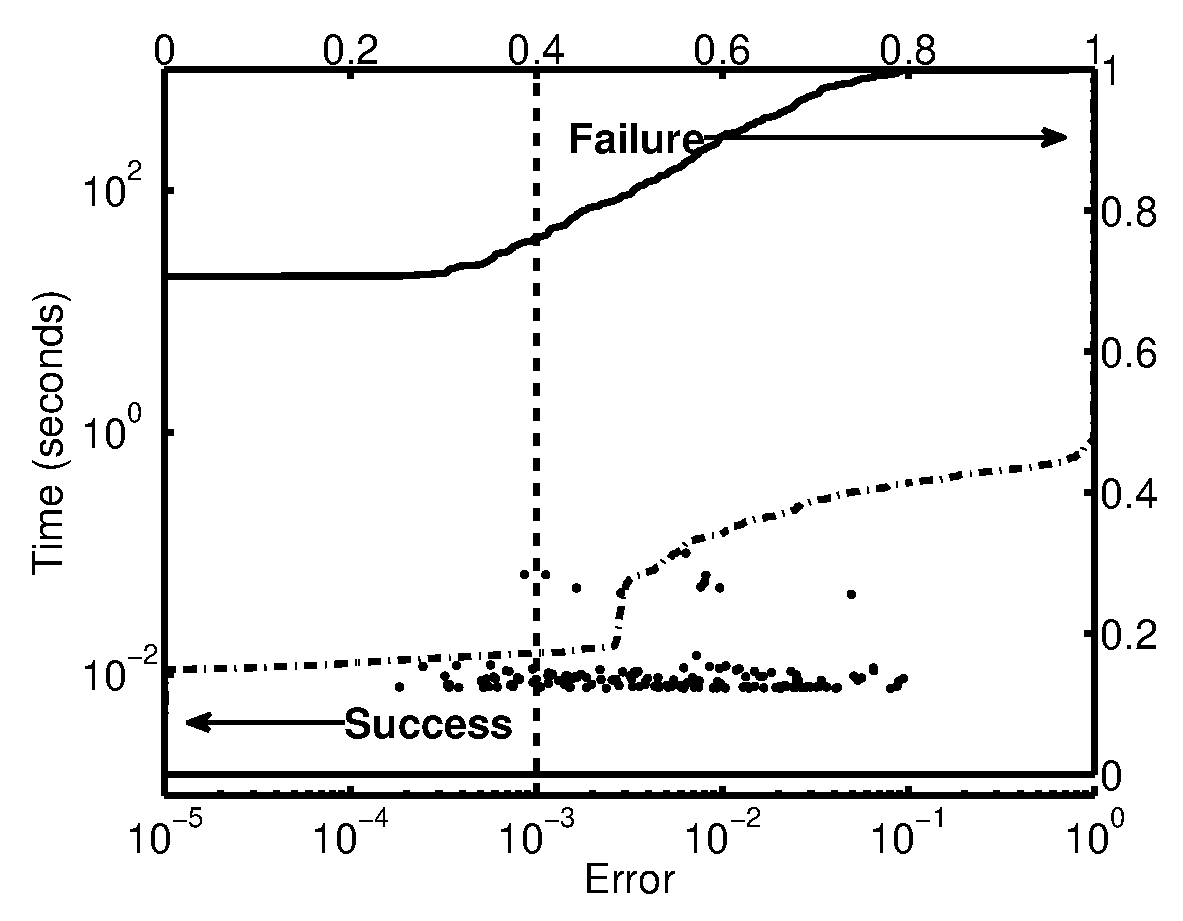
\includegraphics[width=5.7cm]{gaussiand=1chebfunheavyErrTime.eps} \\ {\tt chebfun}  heavy duty\end{minipage}
\begin{minipage}{5.7cm} \centering 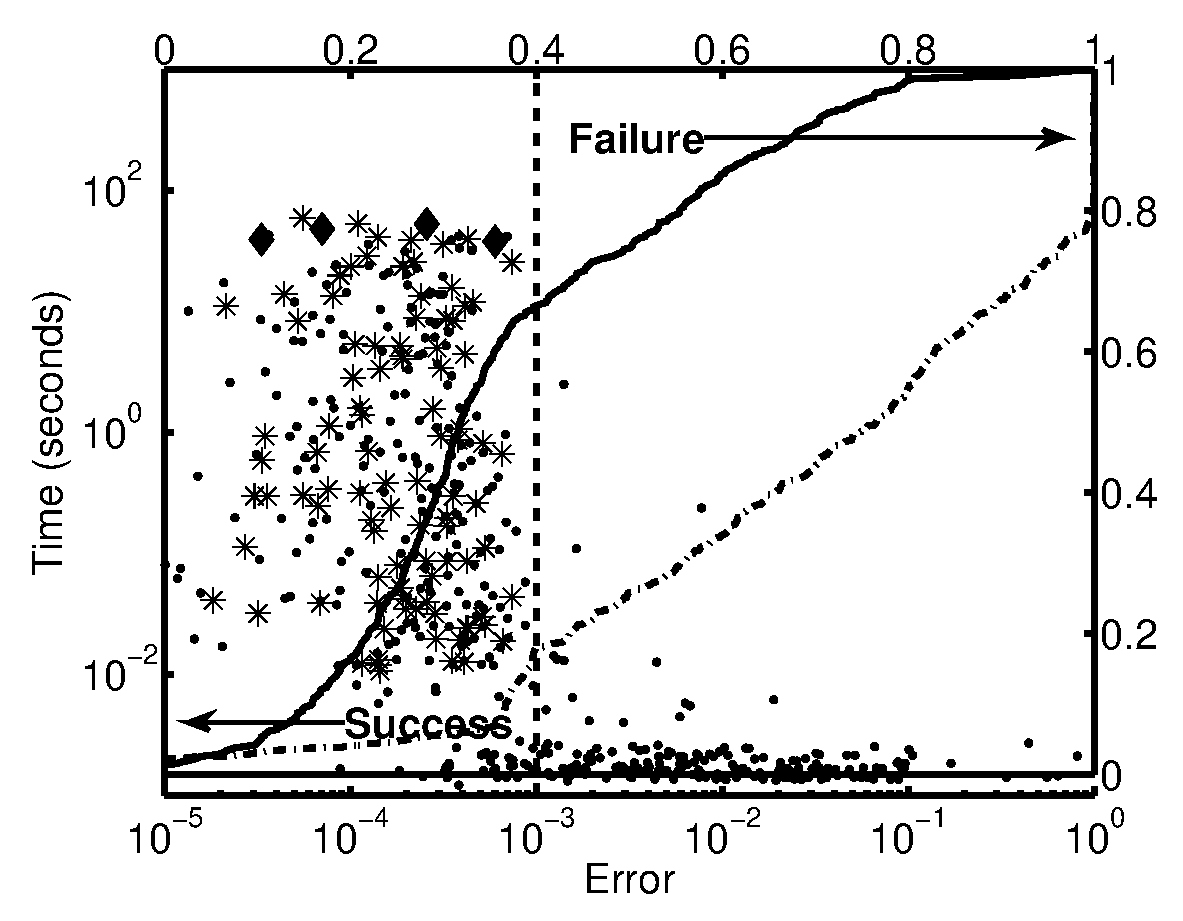
\includegraphics[width=5.7cm]{gaussiand=1iidErrTime.eps} \\ {\tt cubMC} i.i.d. \end{minipage}
\begin{minipage}{5.7cm} \centering 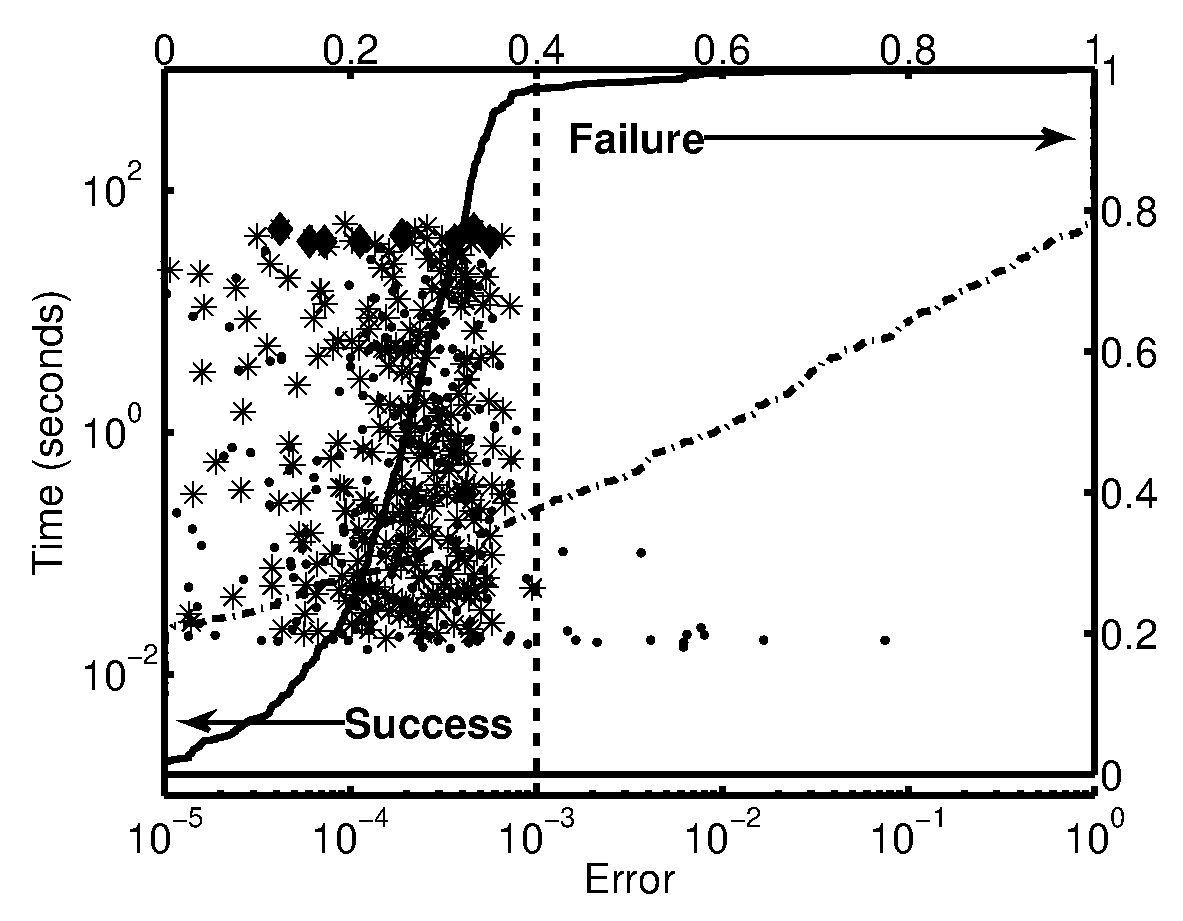
\includegraphics[width=5.7cm]{gaussiand=1iidheavyErrTime.eps} \\ {\tt cubMC} i.i.d. heavy duty\end{minipage}
\begin{minipage}{5.7cm} \centering 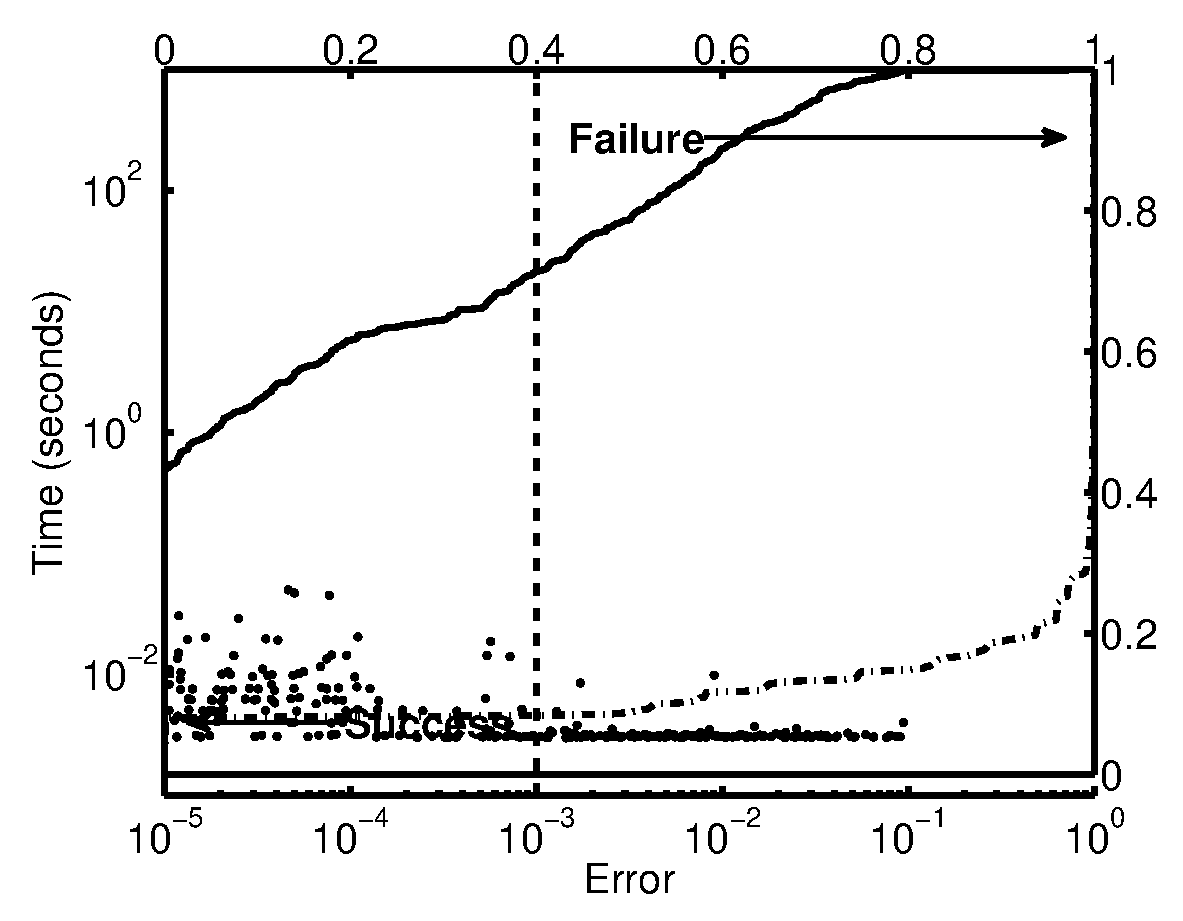
\includegraphics[width=5.7cm]{gaussiand=1SobolErrTime.eps} \\ {\tt cubMC}  Sobol'\end{minipage}
\begin{minipage}{5.7cm} \centering 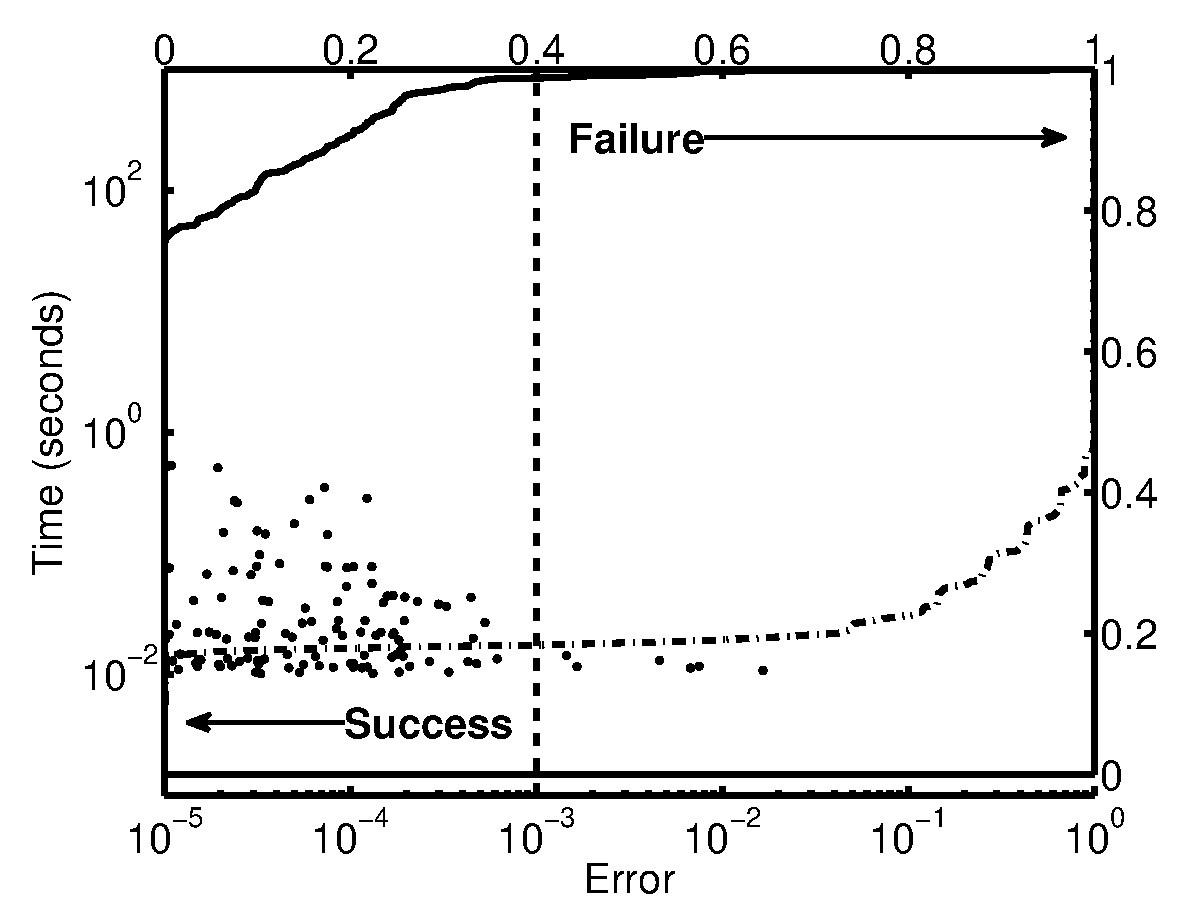
\includegraphics[width=5.7cm]{gaussiand=1SobolheavyErrTime.eps} \\ {\tt cubMC} Sobol' heavy duty \end{minipage}
\caption{Execution times and errors for test function \eqref{GaussianTestFun} for $d=1$ and $\varepsilon=10^{-3}$, and a variety of parameters giving a range of $\sigma(f)$ and $\kappa(f)$. The solid line shows that cumulative distribution of actual errors, and the dot-dashed line shows the cumulative distribution of execution times.  For the {\tt cubMC} i.i.d.\ and i.i.d.\ heavy duty the points labeled * are those for which the Theorem \ref{mainadaptthm} guarantees the error tolerance.\label{GaussianTestFunFig} }
\end{figure}

These $500$ random constructions of $f$ with $d=1$ are integrated over $[0,1]$ with $\rho=1$ (the uniform density function), using {\tt quad},  {\tt quadgk}, and {\tt chebfun}.  For the first two of these algorithms, the specified absolute error tolerance is $\epsilon=0.001$.  The algorithm {\tt chebfun} attempts to do all calculations to near machine precision.  The observed error and execution times are plotted in Figure \ref{GaussianTestFunFig}.  Whereas {\tt chebfun} uses a minimum of $2^3+1=9$ function values, the figure labeled ``{\tt chebfun} heavy duty'' displays the results of requiring chebfun to use at least $2^{10}+1=1025$ function values.  

Figure \ref{GaussianTestFunFig} shows that {\tt quad} and {\tt quadgk} are quite fast, nearly always providing an answer in less that $0.01$ seconds.  Unfortunately, they successfully meet the error tolerance only about $30\%$ of the time for {\tt quad} and $50$--$60\%$ of the time for {\tt quadgk}.  The difficult cases are those where $c_1$ is quite small, and these algorithms miss the sharp peak.  The performance of {\tt chebfun} is similar to that of {\tt quad} and {\tt quadgk}.  The heavy duty version of  {\tt chebfun} fares somewhat better.  
%The {\tt cubMC} algorithm is described in the next section and the results displayed in Figure \ref{GaussianTestFunFig} are described in Section \ref{numerexsec}.

\section{Adaptive Monte Carlo with Guaranteed Error Estimation}

This section describes an adaptive Monte Carlo algorithm based on i.i.d.\ sampling that has probabilistic guarantees on satisfying an absolute error tolerance.  A software implementation of this algorithm, {\tt cubMC}, is being developed by the authors and their collaborators.  Numerical experiments using {\tt cubMC} are shown in Figure \ref{GaussianTestFunFig} above and in Section \ref{numerexsec} below.

\subsection{Reliably Bounding the Variance} To estimate or bound the variance of $Y=f(\vX)$ one must have a finite fourth moment.  The definitions of the variance and kurtosis of $Y$ in Section \ref{statperspsec} may be extended naturally to $f \in \cl_4$ in terms of $\cl_p$ norms defined in \eqref{Lpnormdef} as follows:
\begin{equation*}
\sigma^2=\var(Y) = \var(f) = \norm[2]{f - \mu(f)}^2, \qquad \kappa=\kurt(Y) = \kurt(f) = \frac{\norm[4]{f - \mu(f)}^4}{\norm[2]{f - \mu(f)}^4}.
\end{equation*}
Thus, one may speak about $Y$ or $f$ interchangeably. If $1 \le q \le p$, then by H\"older's inequality,
\begin{align*}\label{LP}
\norm[q]{f} &=\left\{\int_{\reals^d} \abs{f(\vx)}^q \rho(\vx) \, \dif \vx\right\}^{1/q}\\
\nonumber & \le \left\{\int_{\reals^d} \abs{f(\vx)}^p \, \rho(\vx) \, \dif \vx \right\}^{1/p} \left\{\int_{\reals^d} 1^{p/(p-q)} \, \rho(\vx) \, \dif \vx\right\}^{(p-q)/(pq)} = \norm[p]{f}.
\end{align*}
Thus, $\kappa=\kurt(f) \ge 1$, provided $\sigma^2=\var(f)>0$.  For $\sigma^2=\var(f)=0$, one defines $\kappa=\kurt(f)=1$.

As mentioned in \eqref{samplevar}, a practical upper bound on $\sigma^2$ may be obtained in terms of the sample variance.  The justification for this statement is contained in the lemma below. Two well-known probability inequalities that are needed here and later are quoted in the following lemma.

\begin{lemma} \label{ChebCantlem}  Suppose that $Z$ is any random variable with finite second moment.  For any $a >0 $,
\begin{gather*}
\Prob\left[\abs{Z-E(Z)} \ge a \right] \le \frac{\var(Z)}{a^2} \qquad \text{Chebyshev's inequality \citep[6.1c]{LinBai10a}} , \\
\Prob[Z-E[Z] \geq a]\leq \frac{\var(Z)}{a^2+\var(Z)} \qquad
\text{Cantelli's Inequality \citep[6.1e]{LinBai10a}}.
\end{gather*}
\end{lemma}

\begin{lemma} \label{varbdlem}  Suppose that $Y$ is a random variable with finite fourth moment, and with mean $\mu$, variance $\sigma^2$, and kurtosis $\kappa$.  Let $\hv_{n}$ denote the unbiased sample variance based on $n$ i.i.d.\ samples, $Y_1, \ldots, Y_n$ as defined in \eqref{samplevar}.  Then for any $\alpha \in (0,1]$ it follows that
\begin{subequations} \label{sampvarbd}
\begin{gather} \label{sampvarup}
\Prob \left[\frac{\hv_{n}}{1 - \sqrt{\left ( \kappa  - \frac{n-3}{n-1}\right)\left(\frac{1-\alpha}{\alpha n}\right)}} > \sigma^2 \right] \ge 1 - \alpha, \\
\label{sampvarlo}
\Prob \left[\frac{\hv_{n}}{1 + \sqrt{\left ( \kappa  - \frac{n-3}{n-1}\right)\left(\frac{1-\alpha}{\alpha n}\right)}} < \sigma^2 \right] \ge 1 - \alpha.
\end{gather}
\end{subequations}
\end{lemma}

\begin{proof} It is known that the sample variance is an unbiased estimator of the variance, i.e., $E(\hv_n)=\sigma^2$.  It is also known from \cite[(7.16)]{Mil86} that the variance of the sample variance can be expressed in terms of $\sigma^2$ and $\kappa$ as
\[
\var(\hv_n) = \frac{\sigma^4}{n} \left ( \kappa  - \frac{n-3}{n-1} \right).
\]
Choosing
$$a=\sqrt{\var(\hv_n) \frac{1-\alpha}{\alpha} } = \sigma^2\sqrt{\left(\kappa-\frac{n-3}{n-1}\right)\left(\frac{1-\alpha}{\alpha n}\right)} >0,
$$
it follows from Cantelli's inequality (Lemma \ref{ChebCantlem})  that
\begin{multline*}
\Prob\left[\hv_n-\sigma^2 \geq
\sigma^2\sqrt{\left(\kappa-\frac{n-3}{n-1}\right)\left(\frac{1-\alpha}{\alpha n}\right)} \right]  = \Prob\left[\hv_n-\sigma^2 \geq
a \right]\\
 \leq \frac{\var(\hv_n)}{a^2+\var(\hv_n)} 
=\frac{\var(\hv_n)}{\var(\hv_n) \frac{1-\alpha}{\alpha}+\var(\hv_n)}  
=\frac{1}{\left(\frac{1-\alpha}{\alpha}\right)+1}=\alpha.
\end{multline*}
Then \eqref{sampvarup} follows directly.  By a similar argument, applying Cantelli's inequality to the expression $\Prob\left[-\hv_n+\sigma^2 \ge a \right]$ implies  \eqref{sampvarlo}. \qed
\end{proof}

Lemma \ref{varbdlem} provides probabilistic justification to use $\hsigma^2 = \fudge^2 \hv_{n_{\sigma}}$ as a reliable upper bound for $\sigma^2=\var(Y)=\var(f)$.  One can claim that $\Prob(\hsigma^2 \ge \sigma^2) \ge 1-\alpha$ assuming that
\begin{multline}
\frac{1}{1 - \sqrt{\left ( \kappa  - \frac{n_{\sigma}-3}{n_{\sigma}-1}\right)\left(\frac{1-\alpha}{\alpha n_{\sigma}}\right)}} \le \fudge^2
\\
\iff \kappa \le \frac{n_{\sigma}-3}{n_{\sigma}-1} + \left(\frac{ \alpha n_{\sigma}}{1-\alpha}\right) \left(1 - \frac{1}{\fudge^2}\right)^2 =: \kappa_{\max} (\alpha,n_{\sigma},\fudge). \label{kappamaxdef}
\end{multline}

Figure \ref{kurtmaxcompareNfig}a shows how large a kurtosis can be accommodated for a given $n_{\sigma}$, $\alpha$, and variance inflation factor $\fudge=1.5$.  Note that for $n=30$, a common rule of thumb for applying the central limit theorem, even $\alpha=0.1$ gives $\kappa_{\max}$ of only about $2$, which is rather restrictive.

\begin{figure}
\centering
\begin{minipage}{2.1in}
\centering 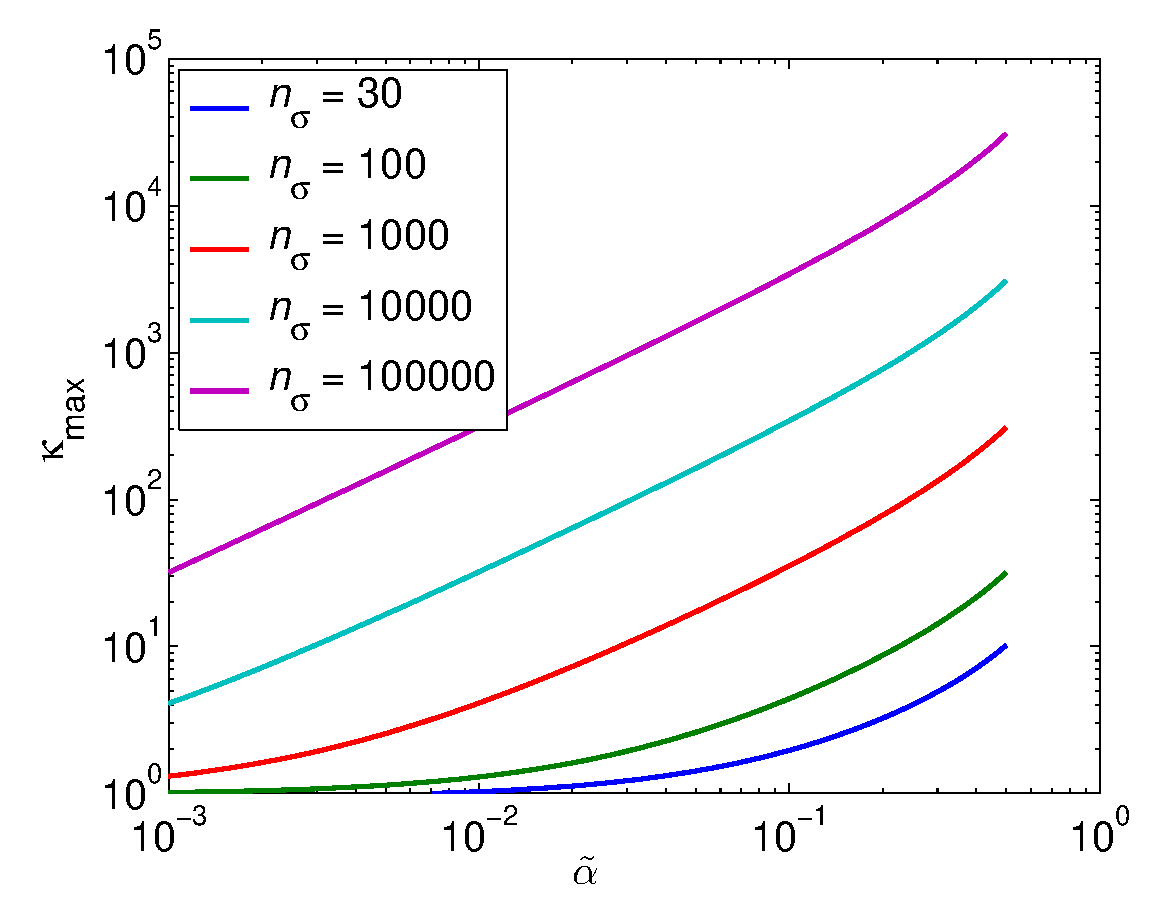
\includegraphics[width=2.1in]{kurtmaxfig.eps} \\
(a)
\end{minipage}
\quad 
\begin{minipage}{2.1in}\centering
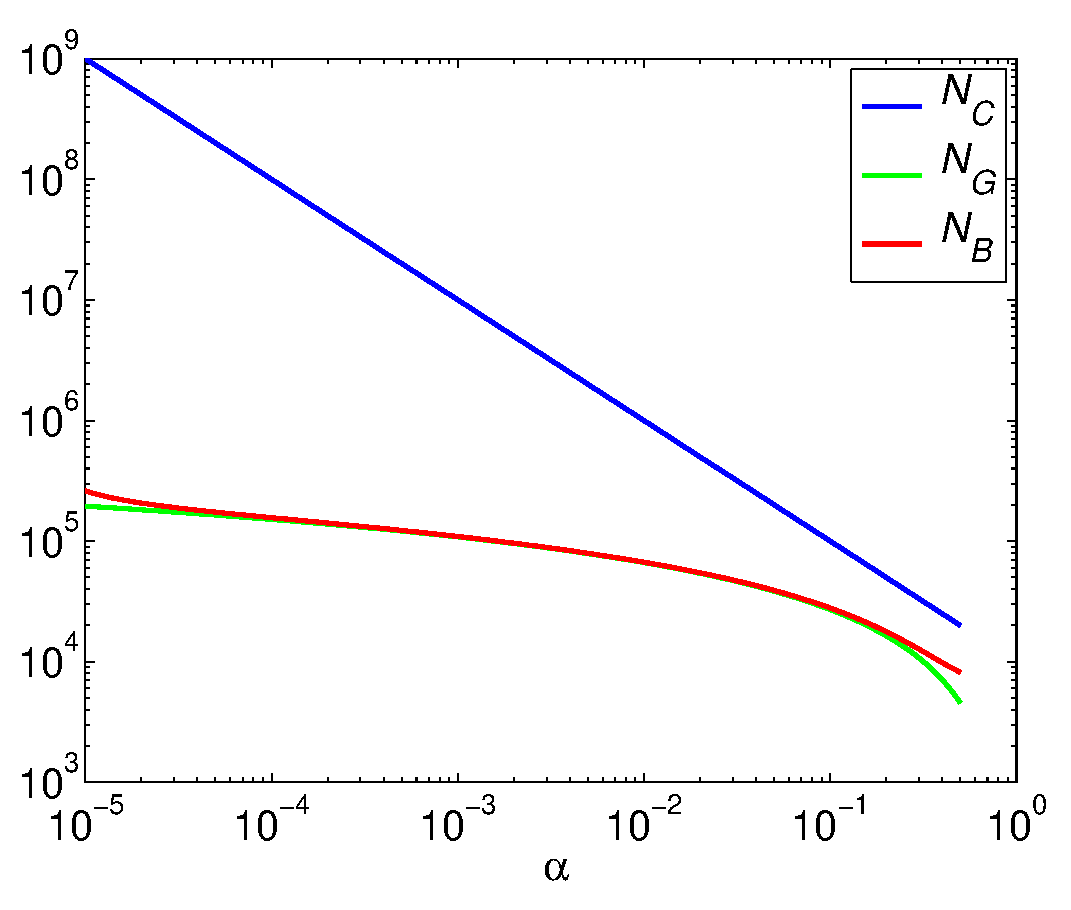
\includegraphics[width=2.1in]{alphacompare.eps}\\
(b)
\end{minipage}
\caption{(a) The maximum kurtosis, $\kappa_{\max}(\alpha,n_{\sigma},1.5)$, as defined in \eqref{kappamaxdef}; (b) comparison of sample sizes $ N_G(0.01,\alpha)$, $N_C(0.01,\alpha)$, and $N_B(0.01,\alpha,\kappa_{\max}^{3/4}(\alpha,1000,1.5))$.\label{kurtmaxcompareNfig}}
\end{figure}

\subsection{Determining the Sample Size} The other issue that needs to be addressed is a tight probabilistic error bound to replace the asymptotic or approximate error bound given by the Central Limit Theorem, \eqref{CLT}.   Chebyshev's inequality implies that the number of function evaluations needed to ensure that $\hmu_n$ satisfies the error tolerance with high probability is
\begin{subequations} \label{ChebErr}
\begin{gather} \label{ChebProbEst}
\Prob\left[\abs{\hmu_n-\mu} \le \varepsilon \right] \ge 1-\alpha \quad \text{for } n \ge N_{C}(\varepsilon/\sigma,\alpha),\ f \in \cl_2,
\intertext{where }
\label{NCdef}
N_{C}(\varepsilon,\alpha) :=\left \lceil \frac{1}{\alpha\varepsilon^2} \right \rceil.
\end{gather}
\end{subequations}
However, this sample size is much larger than that given by the Central Limit Theorem, as shown in Figure \ref{kurtmaxcompareNfig}b.

Since higher order moments of the integrand are required to guarantee an upper bound on the true variance in terms of the sample variance, it is sensible to use these higher order moments to obtain smaller sample sizes.  A smaller sample size than \eqref{NCdef} with a rigorous probabilistic bound can be found by invoking the following inequality. 
\begin{lemma}[Non-uniform Berry-Esseen Inequality] \cite[Theorem 5.16, p. 168]{Pet95a} \label{BE} Let $Y_1,\dots,Y_n$ be i.i.d.\ random variables.  Suppose that
$\mu=E(Y_i)$, $\var(Y_i)=\sigma^2>0$,  and $M=E\abs{Y_i - \mu}^3/\sigma^3 < \infty$.
Then
\[
\abs{\Prob\left[\frac{1}{\sigma\sqrt{n}}\sum_{i=1}^{n}(Y_i-\mu)<x
\right]-\Phi(x)}\leq \frac{A M}{\sqrt{n}(1+\abs{x})^{3}}.
\] for all x,
where $\Phi$ is the cumulative distribution function of a standard Gaussian (normal) random variable, and $A$ is some number satisfying $0.4097\leq A\leq 0.5600$.
\end{lemma}

The right hand side of this inequality bounds how far the probability distribution of sample mean deviates from the Central Limit Theorem approximation.  This right hand side vanishes as either the sample size or $\abs{x}$ tends to infinity. This inequality requires that $Y=f(\vX)$, have a finite third moment, i.e., $f \in \cl_3$, which is a weaker assumption than is needed to bound the variance in terms of the sample variance in Lemma \ref{varbdlem}. Recalling that $Y_i = f(\vX_i)$, $\mu=E(Y_i)$, and $\hmu_n =
(Y_1 + \cdots + Y_n)/n$, this
Berry-Esseen inequality then implies that for positive $x$,
\begin{align} 
\nonumber
\Prob\left[\abs{\hmu_n - \mu} <\frac{\sigma x}{\sqrt{n}}\right]&=\Prob\left[\hmu_n - \mu<\frac{\sigma x}{\sqrt{n}}\right]-\Prob\left[\hmu_n - \mu <-\frac{\sigma x}{\sqrt{n}}\right]\\
\nonumber
&\ge \left[\Phi(x)-\frac{0.56 M}{\sqrt{n}(1+\abs{x})^{3}}\right] -\left[\Phi(-x) + \frac{0.56 M}{\sqrt{n}(1+\abs{x})^{3}}\right]\\
&=1-2\left(\Phi(-x) - \frac{0.56 M}{\sqrt{n}(1+\abs{x})^{3}}\right). \label{BEresult}
\end{align}
Letting $x=\varepsilon\sqrt{n}/\sigma$, the probability of
making an error less than $\varepsilon$ is bounded below by $1-\alpha$, i.e., 
\begin{subequations} \label{proberrcritsampleBE}
\begin{equation}
\Prob[\abs{\hmu_n -\mu}<\varepsilon] \geq 1-\alpha,  \quad \text{provided } n \ge N_B(\varepsilon/\sigma,\alpha,M), \ f \in \cl_3,
\end{equation}
where 
\begin{equation}\label{NB}
N_B(b,\alpha,M) := \min \left \{ n \in \naturals : \Phi\left(-b \sqrt{n}  \right)+\frac{0.56M}{\sqrt{n}\left(1+ b\sqrt{n} \right)^{3}}
\le \frac{\alpha}{2} \right \}.
\end{equation}
\end{subequations}

As shown in Figure \ref{kurtmaxcompareNfig}b, for a range of $\alpha$, the sample size guaranteeing coverage of the confidence interval, $N_B$, is quite close to the sample size for the approximate Central Limit Theorem confidence interval, $N_G$, however, $N_B$ may be somewhat larger for very small or rather large $\alpha$.  In general $N_B$ is significantly smaller than $N_C$, but not always.  A disadvantage of \eqref{proberrcritsampleBE} is that class of integrands, $\cl_3$, is smaller than that in \eqref{ChebErr}, but this typically a small price to pay given the much smaller cost of computation.

The theorem below combines the results on estimating the variance with the sample sizes arising from Chebyshev's inequality and the Berry-Esseen inequality.  These lead to an adaptive Monte Carlo algorithm with a probabilistic error guarantee.

\begin{theorem} \label{mainadaptthm} Specify the following parameters defining the algorithm:
\begin{itemize}
\item sample size for variance estimation, $n_{\sigma} \in \naturals$,
\item inflation factor for variance estimation, $\fudge \in (1,\infty)$,
\item uncertainty tolerance, $\alpha\in (0,1)$, and $\talpha = 1 - \sqrt{1 - \alpha}$, and
\item absolute error tolerance, $\varepsilon \in (0,\infty)$. 
\end{itemize} 
For $\kappa_{\max}=\kappa_{\max}(n_{\sigma},\talpha,\fudge)$, as defined in \eqref{kappamaxdef}, define the cone of integrands functions with bounded kurtosis, $\cc_{\kappa_{\max}}$, according to \eqref{coneintegdef}.  For any $f \in \cc_{\kappa_{\max}}$, compute the sample variance, $\hv_{n_{\sigma}}$ using a simple random sample of size $n_{\sigma}$. Use this to approximate the variance of $f$ by $\hsigma^2 = \fudge^2 \hv_{n_{\sigma}}$ as in \eqref{samplevar}.  Next define a sample size $n = N_{CB}(\varepsilon/\hsigma,\talpha,\kappa_{\max}^{3/4})$, where
\begin{equation} \label{NCBdef}
N_{CB}(b,\alpha,M) := \min\left( N_C(b,\alpha), N_B(b,\alpha,M) \right),
\end{equation} 
$N_C$ is defined in \eqref{NCdef} and  $N_B$ is defined in \eqref{NB}.  Compute $\hmu_n$, the simple Monte Carlo estimator of $\mu$ based on $n$ samples, as in \eqref{simpleMCest}.  A probabilistic absolute error bound is given by
\[
\Prob\left[\abs{\hmu_n-\mu} \le \varepsilon \right] \geq 1-\alpha.
\]
\end{theorem}
\begin{proof} Note that \eqref{LP} implies that the third moment can be bounded in terms of the fourth moment, namely $M$ in Lemma \ref{BE} is no greater than $\kappa^{3/4}$. There are three primary random variables in this algorithm:  the estimated upper bound on the standard deviation, $\hsigma$, the sample size to estimate the mean, $n$, which is an explicit function of $\hsigma$, and the estimated mean, $\hmu_n$. By  \eqref{ChebErr} and \eqref{proberrcritsampleBE} it then follows that  $\Prob\left[\abs{\hmu_n-\mu} \le \varepsilon \right] \geq 1-\talpha$, provided that $\hsigma  \ge \sigma$. Thus, 
\begin{align*}
\Prob\left[\abs{\hmu_n-\mu} \le \varepsilon \right] &
= E_{\hsigma} \left\{\Prob\left[\abs{\hmu_n-\mu} \le \varepsilon \ | \ \hsigma \right] \right\} \\
& \ge E_{\hsigma} \left\{(1-\talpha) 1_{[\sigma,\infty)}(\hsigma) \right\}\\
& \ge (1-\talpha) (1-\talpha) = 1-\alpha,
\end{align*}
since $\hsigma \ge \sigma$ with probability $1-\talpha$ by \eqref{kappamaxdef}.  \qed
\end{proof}

\begin{remark} If one is willing to invest $n_\sigma$ samples to estimate $\sigma$, it makes practical sense to to choose the sample size for the sample mean at least that large, i.e, 
\[
n = \max(n_{\sigma},N_{CB}(\varepsilon/\hsigma,\talpha,\kappa_{\max}^{3/4})).
\]
By the error bound following from Chebyshev's inequality, \eqref{ChebErr}, this means that the probabilistic absolute error bound in Theorem \ref{mainadaptthm} also holds for integrands, $f$, lying in the ball $\cb_{\sigma_{\max}}$, defined in \eqref{ballintegdef}, where $\sigma_{\max} = \varepsilon \sqrt{\alpha n_{\sigma}}$.
\end{remark}


\subsection{Cost of the Algorithm}  The sample size of the adaptive algorithm defined in Theorem \ref{mainadaptthm} is a random variable, and so the cost of this algorithm might best be defined defined probabilistically.  Moreover, the cost depends strongly on $\sigma$ as well as the $\varepsilon$, and its definition should reflect this dependence. 

Let $A$ be any random algorithm defined for a set of integrands $\cf$ that takes as its input an error tolerance, $\varepsilon$, an uncertainty level, $\alpha$, and a  procedure for computing values of $f \in \cf$.  The algorithm then computes an approximation to the integral, $A(f,\varepsilon,\alpha)$.  This approximation is based solely on  $f(\vx_1), \ldots, f(\vx_n)$, where the choice of each $\vx_i$ may depend iteratively on $(\vx_1,f(\vx_1)), \ldots, (\vx_{i-1},f(\vx_{i-1}))$, and the decision to stop with $n$ data depends on all function data collected, up to and including the $n^{\text{th}}$.  The cost of this algorithm for this set of inputs is denoted $\cost(A,\varepsilon,\alpha,f)$, is the number of function values, $n$, which as noted is a random variable.  The probabilistic cost of the algorithm, with uncertainty $\beta$, for integrands of variance no greater than $\sigma^2_{\max}$ is defined as 
\begin{equation}
\cost(A,\varepsilon,\alpha,\beta,\cf,\sigma_{\max}) := \sup_{\substack{f \in \cf\\ \var(f)\le \sigma^2} } \min\left\{N : \Prob[\cost(A,\varepsilon,\alpha,f) \le N] \ge 1-\beta  \right \}.
\end{equation}

The cost of the particular adaptive Monte Carlo algorithm defined in Theorem \ref{mainadaptthm}, denoted $\aMC$, for the cone of integrands $\cc_{\kappa_{\max}}$ is
\begin{equation}
\cost(\aMC,\varepsilon,\alpha, \beta, \cc_{\kappa_{\max}}, \sigma_{\max}) := \sup_{\substack{f \in \cc_{\kappa_{\max}}\\ \var(f)\le \sigma^2_{\max}} } \min\left\{N : \Prob(n_{\sigma} + n \le N) \ge 1-\beta  \right \}.
\end{equation}
Since $n_{\sigma}$ is fixed, bounding this cost depends on bounding $n$, which depends on $\hsigma$ as given by Theorem \ref{mainadaptthm}.  Moreover, $\hsigma$ can be bounded above using \eqref{sampvarlo} in Lemma \ref{varbdlem}.  For $f \in \cc_{\kappa_{\max}}$, 
\begin{align*}
1-\beta & \le \Prob\left[\hv_{n_{\sigma}} < \sigma^2 \left\{1 + \sqrt{\left ( \kappa  - \frac{n_{\sigma}-3}{n_{\sigma}-1}\right)\left(\frac{1-\beta}{\beta n_{\sigma}}\right)}\right\} \right] \\
& \le \Prob\left[\hsigma^2 = \fudge^2 \hv_{n_{\sigma}} < \fudge^2\sigma^2 \left\{1 + \sqrt{\left ( \kappa_{\max}(n_{\sigma},\talpha,\fudge)  - \frac{n_{\sigma}-3}{n_{\sigma}-1}\right)\left(\frac{1-\beta}{\beta n_{\sigma}}\right)}\right\} \right] \\
%& = \Prob\left[\hsigma^2 < \fudge^2\sigma^2 \left\{1 + \sqrt{\left(\frac{ \talpha }{1-\talpha}\right) \left(\frac{1-\beta}{\beta}\right) \left(1 - \frac{1}{\fudge^2}\right)^2}\right\} \right] \\
& = \Prob\left[\hsigma^2 < \sigma^2 \gamma^2(\talpha,\beta,\fudge) \right],
\end{align*}
where
\[
\gamma^2(\talpha,\beta,\fudge) := \fudge^2 \left\{1 + \sqrt{\left(\frac{ \talpha }{1-\talpha}\right) \left(\frac{1-\beta}{\beta}\right) \left(1 - \frac{1}{\fudge^2}\right)^2}\right\} > 1.
\]
Noting that $N_{CB}(\cdot,\alpha,M)$ is a non-increasing function allows one to derive the following upper bound on the cost of the adaptive Monte Carlo algorithm.

\begin{theorem} \label{costtheorem} The adaptive Monte Carlo algorithm based on i.i.d.\ sampling described in Theorem \ref{mainadaptthm}, denoted $\aMC$, has a probabilistic cost bounded above by 
\begin{equation*}
\cost(\aMC,\varepsilon,\alpha, \beta, \cc_{\kappa_{\max}}, \sigma_{\max})
\le n_{\sigma} + N_{CB}(\varepsilon/(\sigma_{\max}\gamma(\talpha,\beta,\fudge)),\talpha,\kappa_{\max}^{3/4}).
\end{equation*} 
\end{theorem}

The cost of the adaptive Monte Carlo algorithm $\aMC$ is roughly proportional to $\sigma^2_{\max}\varepsilon^{-2}$.  The set $\cc_{\kappa_{\max}}$ contains integrands with arbitrarily large variance, $\sigma^2=\var(f)$, and thus with potentially arbitrarily large algorithmic cost.  On the other hand, since the algorithm is adaptive, the cost may be small if $\sigma^2$ is small.  The upper bound in Theorem \ref{costtheorem} certainly scales with the $\sigma^2_{\max}$ as one might hope if $\sigma^2_{\max}$ were known.  The variable cost of the algorithm for integrands in $\cc_{\kappa_{\max}}$ is actually an advantage, rather than a drawback, of this analysis.  One need not make any a priori assumptions about the size of the integrand, $\sigma$, only about its kurtosis, $\kappa$, which is unchanged when the integrand is multiplied by an arbitrary nonzero constant.

\section{Numerical Examples with $\aMC$} \label{numerexsec}

Figure \ref{GaussianTestFunFig} shows timing and observed errors for the adaptive algorithm, $\aMC$, with i.i.d.\ sampling, as described in the previous section.  The parameters chosen are $\epsilon=0.001$, $\alpha=5\%$, and  $\fudge=1.5$.  For the plot on the left, $n_\sigma=2^{10}=1024$, which corresponds to  $\kappa_{\max}=9.2$.  For the heavy duty plot on the right, $n_\sigma=2^{17}=131\ 072$, which corresponds to  $\kappa_{\max}=1052$. In both of these plots the points labeled with a * are those for which $\kappa(f) \le \kappa_{\max}$ and so Theorem \ref{mainadaptthm} guarantees that the answer is correct $1-\alpha= 95\%$ of the time.  For these plots all of the points labeled * fall within the prescribed error tolerance.  For $\aMC$ i.i.d.\ heavy duty plot $\kappa_{\max}$ is larger, so there are more points for which the guarantee holds.  Those points labeled with a dot, are those for which $\kappa(f) > \kappa_{\max}$, and so no guarantee holds. The points labeled with a square are those for which \aMC attempts to exceed the cost budget, i.e., it wants to choose $n$ such that $(n_{\sigma}+n)d > N_{\max}=10^9$. 

The {\tt cubMC} algorithm performs somewhat more robustly than {\tt quad}, {\tt quadgk}, and {\tt chebfun}, because \aMC does requires a very low degree of smoothness and makes a fairly large minimum sample.  The more important point is that \aMC has a guarantee, where to our knowledge, the other routines do not.

Figure \ref{GaussianTestFunFig} also exhibits the results of using \aMC with scrambled Sobol' sampling \citep{Owe95,Owe96,Owe97,Mat98,HonHic00a,DicPil10a}, i.e., the sample mean,  $\hmu_n$ is based on sampling the integrand on a Sobol' net with $n$ points.  Since the points of the Sobol' net are purposefully correlated, the error of $\hmu_n$ does not depend on $\var(f)$, but on some measure of variation of $f$ (see \citep{Owe95,Owe96,Owe97,DicPil10a}) that is difficult to estimate in practice.  Tony Warnock and John Halton proposed the following error bound estimate, called the quasi-standard error \citep{Hal05a,Owe06a}:
\begin{equation} \label{qsedef}
\qse(f;m) = \sqrt{\frac{1}{m(m-1)} \sum_{j=1}^m  [\hmu^{(j)}_n - \hmu_n]^2}.
\end{equation}
where $\hmu^{(j)}$ corresponds to the sample mean of the function values for the $j^{\text{th}}$ partition out of the Sobol' net.  In \aMC the error of $\hmu_n$ is assumed to be no greater than  $\fudge \qse(f;m)$ with $m=8$ and $\fudge=1.5$.  The number of samples, $n$, is doubled until $\fudge \qse(f;m) \le \varepsilon$.  Unfortunately, there is no theory yet that intuitively describes the cone of integrands for which this stopping criterion guarantees that the error tolerance is met.  This is an area of ongoing research.

Clearly, from Figure \ref{GaussianTestFunFig}, the Sobol' sampling option is more reliable and takes less time than the i.i.d.\ option of \aMC.  This is due primarily to the fact that in dimension one, Sobol' sampling is equivalent to stratified sampling, where the points are more evenly spread.

Figure \ref{GaussianTestFunHDFig} repeats the simulation shown in Figure \ref{GaussianTestFunFig} for the same test function \eqref{GaussianTestFun}, but now with $d=2, \ldots, 8$ chosen randomly and uniformly.  For this case the univariate integration algorithms are inapplicable, but \aMC with both sampling schemes, i.i.d.\ and Sobol', can be used.  There are more cases where the \aMC tries to exceed the maximum sample size allowed, but the behavior seen for $d=1$ still generally apply.  

\begin{figure}
\centering
\begin{minipage}{5.7cm} \centering 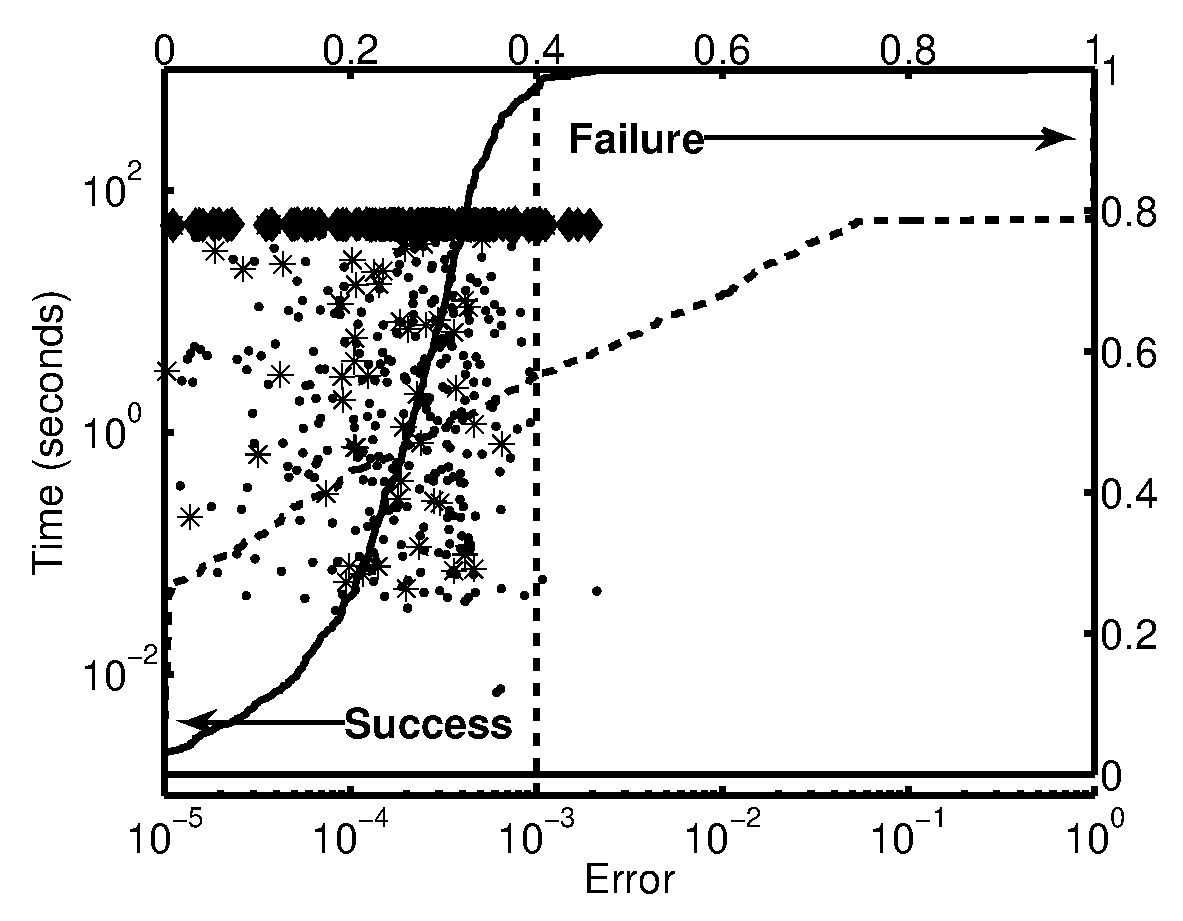
\includegraphics[width=5.7cm]{gaussiand=7iidErrTime.eps} \\ {\tt cubMC} i.i.d. \end{minipage}
\begin{minipage}{5.7cm} \centering 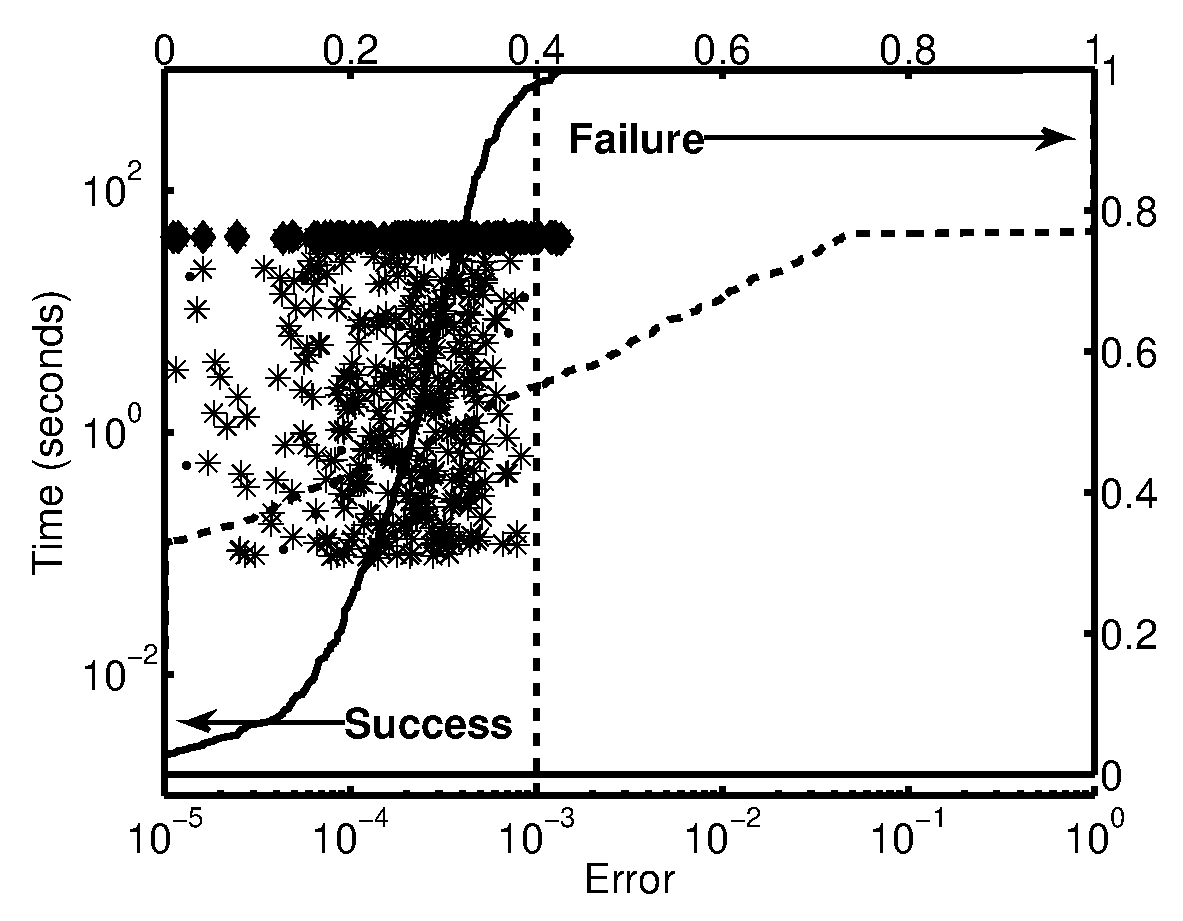
\includegraphics[width=5.7cm]{gaussiand=7iidheavyErrTime.eps} \\ {\tt cubMC} i.i.d heavy duty \end{minipage}
\begin{minipage}{5.7cm} \centering 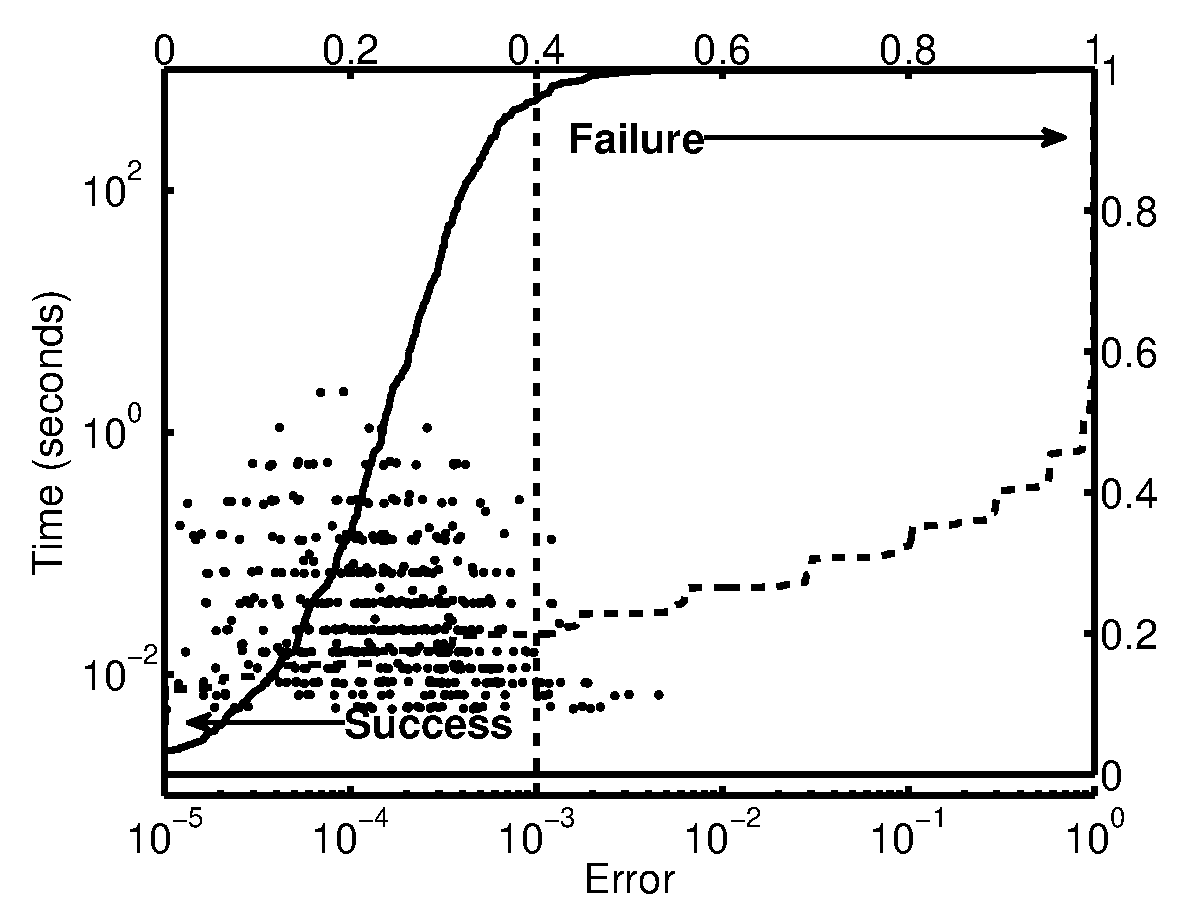
\includegraphics[width=5.7cm]{gaussiand=7SobolErrTime.eps} \\ {\tt cubMC} Sobol' \end{minipage}
\begin{minipage}{5.7cm} \centering 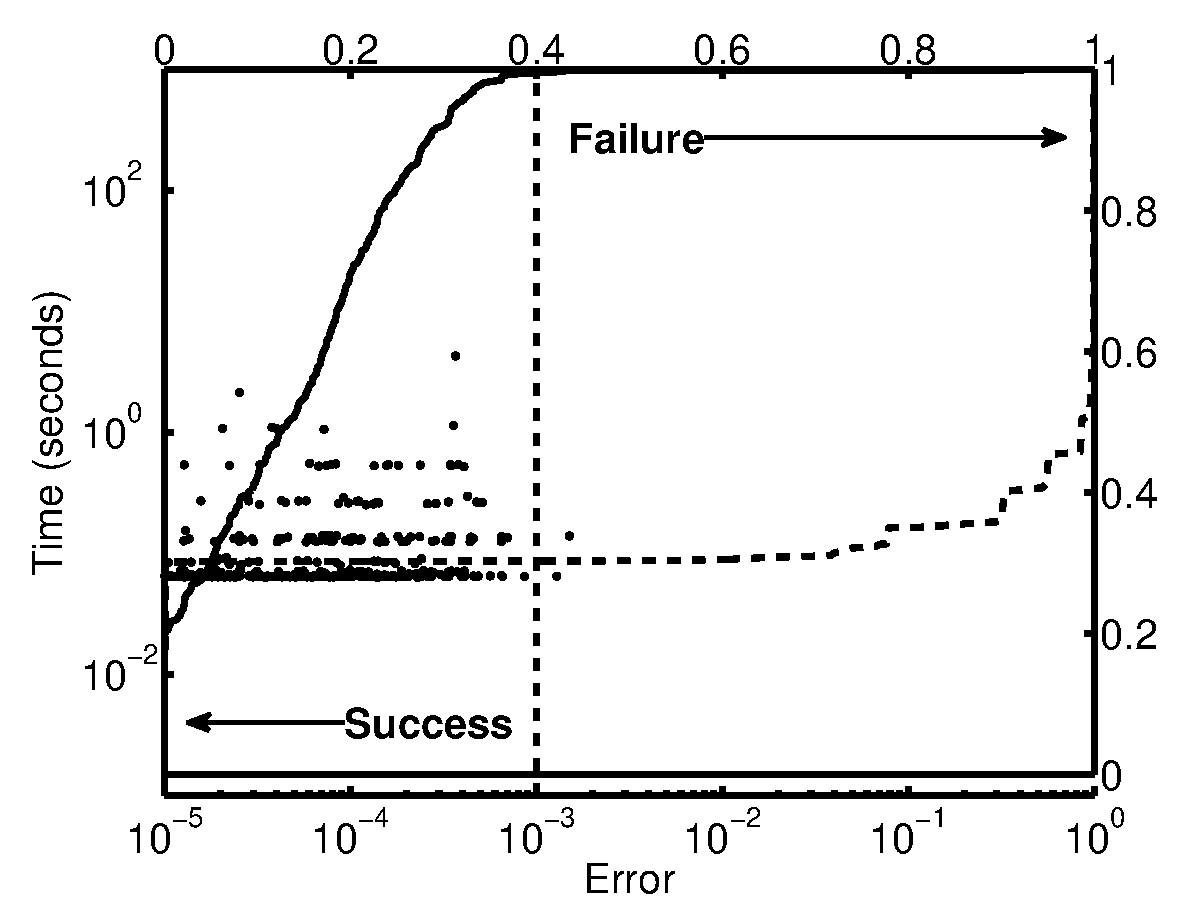
\includegraphics[width=5.7cm]{gaussiand=7SobolheavyErrTime.eps} \\ {\tt cubMC} Sobol' heavy duty \end{minipage}
\caption{Execution times and errors for test function \eqref{GaussianTestFun} for $d=2, \ldots, 8$ and $\varepsilon=10^{-3}$, with the rest of the parameters as in Figure \ref{GaussianTestFunFig}.\label{GaussianTestFunHDFig}}
\end{figure}

{\bf We will put one more finance example here.}

\section{A General Error Criterion} \label{relerrsec}

In many practical situations, one needs to approximate the integral with a certain relative accuracy.  For example, one wants an answer that is correct to three significant digits.  In this case, given a tolerance, $\varepsilon$, and a significance level $\alpha$, with $\varepsilon, \alpha \in (0, 1)$, one seeks a random $\tmu$ such that 
\begin{equation*} \label{relerrcrit}
\Prob\left[\abs{\frac{\tmu-\mu}{\mu}} \le \varepsilon \right] \geq 1-\alpha.
\end{equation*}
A more general form of this criterion would be
\begin{equation} \label{genrelerrcrit}
\Prob\left[\frac{\abs{\tmu-\mu}} {1-\theta + \theta\abs{\mu}} \le \varepsilon \right] \geq 1-\alpha.
\end{equation}
for some fixed $\theta \in [0,1]$, where $\theta=0$ corresponds to absolute error, and $\theta = 1$ corresponds to relative error.  Clearly, one must have $(1-\theta) + \abs{\mu}\ne0$ for such a statement to be possible.  

If $\varepsilon_{A} \ge 0$ is an absolute error tolerance, and $\varepsilon_{R} \ge 0$ is a relative error tolerance, then letting 
\[
\varepsilon = \frac{\varepsilon_{A}\varepsilon_{R}}{\theta \varepsilon_{A} + (1-\theta) \varepsilon_{R}},
\]
it follows that for all $\theta \in [0,1]$,
\[
[1-\theta + \theta \abs{\mu}]\varepsilon = (1-\gamma)\varepsilon_{A} + \gamma \varepsilon_{R} \abs{\mu} \le \max(\varepsilon_{A},\varepsilon_{R} \abs{\mu}),
\]
where
\[
\gamma = \frac{\theta \varepsilon_{A}}{\theta \varepsilon_{A} + (1-\theta) \varepsilon_{R}} \in [0,1].
\]
Thus, error criterion  \eqref{genrelerrcrit} implies that one has satisfied either an absolute or a relative error criterion, 
\[
\Prob\left[\frac{\abs{\tmu-\mu}} {1-\theta + \theta\abs{\mu}} \le \varepsilon \right] \geq 1-\alpha \implies \Prob\left[\abs{\tmu-\mu} \le \varepsilon_A \text{ or } \abs{\tmu-\mu} \le \abs{\mu}\varepsilon_R \right] \geq 1-\alpha.
\]
A value of $\gamma$ close to zero implies a preference to fulfill the absolute error criterion while a value of $\gamma$ close to one implies a preference to fulfill the relative error criterion.

Obtaining a confidence interval of the form \eqref{genrelerrcrit}, proceeds in three stages: i) obtaining an upper bound on $\sigma^2$, ii) obtaining a lower bound on $1-\theta + \theta\abs{\mu}$, and iii) then using these to obtain \eqref{genrelerrcrit}.  What differs from the absolute error case is step ii).  For this step it is noted that
\begin{multline} \label{relerrcritd}
\Prob\left[\abs{\hmu-\mu} \le \hvareps \right] \ge 1-\alpha \implies \Prob[\max(\abs{\hmu}-\hvareps,0) \le \abs{\mu} \le \abs{\hmu}+\hvareps] \ge 1-\alpha \\
\implies \Prob[1-\theta + \theta\max(\abs{\hmu}-\hvareps,0) \le 1-\theta + \theta\abs{\mu} \le 1-\theta + \theta(\abs{\hmu}+\hvareps)] \ge 1-\alpha.
\end{multline}
Although one might be happy the left side of this inequality being positive, if it is too much smaller than the right side, then one might be eventually expending too much extra work in step iii).  Thus, it makes sense to require 
\begin{gather*}
1-\theta + \theta\max(\abs{\hmu}-\hvareps,0) \ge \hdelta [1-\theta + \theta(\abs{\hmu}+\hvareps)] \\
\iff \hvareps = \begin{cases}
\displaystyle \frac{(1-\hdelta)(1-\theta)}{\hdelta \theta} -\abs{\hmu}, & 
\displaystyle 0 \le \abs{\hmu}  < \frac{(1-\hdelta)(1-\theta)}{2 \hdelta \theta},
 \\[2ex]
\displaystyle \frac{1-\hdelta}{1+\hdelta} \left[\frac{1-\theta}{\theta} +\abs{\hmu}\right], & 
\displaystyle \frac{(1-\hdelta)(1-\theta)}{2 \hdelta \theta} \le \abs{\hmu}  < \infty.
\end{cases}
\end{gather*}
This is done iteratively in the algorithm described in Theorem \ref{relerradaptthm} below.  One needs to prevent $\hvareps$ from becoming too small.  This means that $\hdelta$ should kept away from $1$, which means that the lower bound on $1-\theta + \theta\abs{\mu}$ is allowed to be somewhat smaller than the upper bound.  Preventing $\hvareps$ from becoming too small also means that $1-\theta + \abs{\hmu}$ cannot be too small. This may be unavoidable if one is interested in relative error $\theta=1$, and the true answer, $\mu$, is small.

Some notation is needed for this theorem.  For any fixed $\alpha \in (0,1)$, and $M>0$, define the inverse of the functions $N_C(\cdot,\alpha)$, $N_B(\cdot,\alpha,M)$, and $N_{CB}(\cdot,\alpha,M)$,
%\begin{subequations} \label{probadapterrcritBE}
\begin{gather*}\label{NCinv}
N_C^{-1}(n,\alpha) := \frac{1}{\sqrt{n \alpha}}, \\
\label{NBinv*}
N_B^{-1}(n,\alpha,M) := \min \left \{ b>0 : \Phi\left(-b \sqrt{n}  \right)+\frac{0.56M}{\sqrt{n}\left(1+ b\sqrt{n} \right)^{3}}
\le \frac{\alpha}{2} \right \}, \\
\label{NCBinv*}
N_{CB}^{-1}(n,\alpha,M) := \min(N_C^{-1}(n,\alpha),N_B^{-1}(n,\alpha,M)).
\end{gather*}
It then follows then by Chebyshev's inequality and the Berry-Esseen Inequality (see \eqref{BEresult}) that 
\begin{equation*}
\Prob[\abs{\hmu_n -\mu}<\hvareps] \geq 1-\alpha, \quad \text{provided } \ f \in \cc_{\kappa_{\max}}, \text{ where }\hvareps=\sigma(f) N_{CB}^{-1}(n,\alpha,\kappa_{\max}^{3/4}), 
\end{equation*} 
%\end{subequations}
and $\sigma(f)=\sqrt{\var(f)}$ is the standard deviation of the integrand.  Given a significance level, $\alpha \in (0,1)$, let $\alpha_{\sigma}, \alpha_{\mu}, \alpha_1,  \alpha_2, \ldots$ be an infinite sequence of positive numbers all less than one, such that 
\begin{equation} \label{alphaseq}
(1-\alpha_{\sigma})(1-\alpha_{\mu})(1-\alpha_1)(1-\alpha_2) \cdots = 1-\alpha.
\end{equation}
For example, one might choose $\alpha_{\sigma},\alpha_{\mu},$ and $\halpha$ such that $(1-\alpha_{\sigma})(1-\alpha_{\mu})(1-\halpha)=1-\alpha$, and then 
\begin{equation} \label{alphaseqex}
\alpha_{i} = 1-(1-\halpha)^{(a-1)a^{-i}}, \ i\in \naturals, \quad \text{where} \  a \in (1,\infty).
\end{equation}

\begin{theorem} \label{relerradaptthm} Specify the following parameters defining the algorithm:
\begin{itemize}
\item sample size for variance estimation, $n_{\sigma} \in \naturals$,
\item initial sample size for mean estimation, $n_1 \in \naturals$,
\item variance inflation factor for variance estimation, $\fudge \in (1,\infty)$, 
\item factors for Step 2, $\hdelta, \delta, \tdelta \in (0,1)$, with $\delta < \tdelta$.
\item uncertainty tolerance, $\alpha\in (0,1)$, and a sequence $\alpha_{\sigma}, \alpha_{\mu}, \alpha_1,  \alpha_2, \ldots$ satisfying \eqref{alphaseq}, 
\item the parameter $\theta \in [0,1]$, used to define the general error criterion \eqref{genrelerrcrit}, and
\item the error tolerance, $\varepsilon >0$. 
\end{itemize} 
Let $\kappa_{\max}=\kappa_{\max}(n_{\sigma},\alpha_{\sigma},\fudge)$ as defined in \eqref{kappamaxdef}.  For any $f$ lying in the cone of functions with bounded kurtosis, $\cc_{\kappa_{\max}}$, do the following:
\begin{enumerate}
%\renewcommand{\labelenumi}{\alph{enumi})}
\item {\bf Bounding the variance of the integrand from above.} Compute the sample variance, $\hv_{n_{\sigma}}$ using a simple random sample of size $n_{\sigma}$. Use this to approximate the variance of $f$ by $\hsigma^2 = \fudge^2 \hv_{n_{\sigma}}$, as in \eqref{samplevar}. Compute the width of initial the confidence interval for the mean, $\hvareps_1=\hsigma N_{CB}^{-1}(n_1,\alpha_1,\kappa_{\max}^{3/4})$.

\item \label{boundcstep} {\bf Bounding the denominator in the error criterion  from below.} For $i=1, 2, \ldots$, do the following:

\begin{enumerate}

\item Compute the sample average $\hmu_{n_i}$ using a simple random sample that is independent of those used to compute $\hv_{n_{\sigma}}$ and $\hmu_{n_1}, \ldots, \hmu_{n_{i-1}}$.

\item Compute $\fc=1-\theta + \theta\max(\abs{\hmu_{n_i}}-\hvareps_{i},0)$, a confident lower bound on $1-\theta + \theta\abs{\mu}$, according to \eqref{relerrcritd}.  If $\fc \ge \delta [1 - \theta + \theta(\abs{\hmu_{n_i}} + \hvareps)]$, then $\fc$ is large enough.  Set $\tau=i$ and go to Step \ref{hmufinalstep}.

\item \label{newhvarepsstep} Else, compute the next tolerance for the sample mean
\begin{gather*}
\hvareps_{0} = \begin{cases}
\displaystyle \frac{(1-\hdelta)(1-\theta)}{\hdelta \theta} -\abs{\hmu_{n_i}}, & 
\displaystyle 0 \le \abs{\hmu_{n_i}}  < \frac{(1-\hdelta)(1-\theta)}{2 \hdelta \theta},
 \\[2ex]
\displaystyle \frac{1-\hdelta}{1+\hdelta} \left[\frac{1-\theta}{\theta} +\abs{\hmu_{n_i}}\right], & 
\displaystyle \frac{(1-\hdelta)(1-\theta)}{2 \hdelta \theta} \le \abs{\hmu_{n_i}}  < \infty,
\end{cases}\\
\hvareps_{i+1} = \max(\min(\hvareps_0, \tdelta \hvareps_i), \delta \hvareps_i).
\end{gather*}


\item Define the next sample size, $n_{i+1} = N_{CB}(\hvareps_{i+1}/\hsigma,\alpha_{i+1},\kappa_{\max}^{3/4})$,
increase $i$ by one, and go to step a). 

\end{enumerate}

\item \label{hmufinalstep} {\bf Computing the sample mean to sufficient accuracy.} Compute the sample size  $n = N_{CB}(\fc \varepsilon/\hsigma,\alpha_\mu,\kappa_{\max}^{3/4})$. Compute $\tmu=\hmu_{n}$ using a simple random sample that is independent of those used to compute $\hv_{n_{\sigma}}$ and $\hmu_{n_1}, \ldots, \hmu_{n_{\tau}}$. Terminate the algorithm.

\end{enumerate}
If this algorithm terminates, then the general error criterion, \eqref{genrelerrcrit}, is satisfied.

\end{theorem}

\begin{proof} In this algorithm there are a number of important random variables:  the estimated upper bound on the standard deviation, $\hsigma$, the sample sizes $n_1, \ldots, n_\tau, n$, the number of iterations, $\tau$, required to get a good  lower bound $\fc$, and the final estimate of the mean $\tmu=\hmu_n$. These sample means are conditionally independent given the sequence of sample sizes.  The probability that the final confidence interval is correct, is then no less than the probability that all of the confidence intervals are correct, conditioned on the sample sizes.  Specifically,
\begin{align*}
\Prob\left[\frac{\abs{\tmu-\mu}} {1-\theta + \theta\abs{\mu}} \le \varepsilon \right] & 
\ge \Prob\left[\abs{\hmu_{n}-\mu} \le \fc \varepsilon \ \& \ \fc\le 1-\theta + \theta\abs{\mu} \right] \\
& = E \left\{\Prob\left[\abs{\hmu_{n}-\mu} \le \fc \varepsilon \ \& \ \abs{\hmu_{n_{\tau}}-\mu} \le \hvareps_\tau \ | \ \hsigma, \tau, n_1, \ldots, n_{\tau},n \right] \right\} \\
& \ge E \left\{\Prob\left[\abs{\hmu_{n}-\mu} \le \fc \varepsilon \ \& \ \abs{\hmu_{n_{i}}-\mu} \le \hvareps_i \ \forall i \ | \ \hsigma, \tau, n_1, \ldots, n_{\tau} \right] \right\} \\
& \ge E_{\hsigma} \left\{[(1-\alpha_\mu)(1-\alpha_1) )(1-\alpha_2) \cdots ] 1_{[\sigma,\infty)}(\hsigma) \right\}\\
& \ge (1-\alpha_{\sigma}) (1-\alpha_\mu) (1-\alpha_1)(1-\alpha_2) \cdots = 1-\alpha. \qquad \qed
\end{align*}
\end{proof}

\begin{remark} Step \ref{boundcstep} in this algorithm is not needed for the case of pure absolute error $\theta=0$, because $\fc=1$ automatically, which is large enough.  As suggested earlier, a difficulty may arise if $\mu \approx 0$ and $\theta \approx 1$, in which the algorithm may fail to converge in a reasonable number of steps and overall sample size.  Step \ref{newhvarepsstep} has safeguards against making $\hvareps_{i+1}$ too small compared to $\hvareps_{i}$, but this may also increase the number of iterations, $\tau$, necessary for completion of Step \ref{boundcstep}.  Because it is difficult to knowing how large $\tau$ is for a given integrand, there is no rigorous bound on the cost of this algorithm yet.
\end{remark}

\section{Discussion}

Put something here.


\section*{Acknowledgements} The authors gratefully acknowledge discussions with Erich Novak and Henryk Wo\'zniakowski.  The plots of the univariate fooling functions were prepared with the help of Nicholas Clancy and Caleb Hamilton.

\bibliographystyle{spbasic}
\bibliography{FJH22,FJHown22}
\end{document}
